%++++++++++++++++++++++++++++++++++++++++
% Don't modify this section unless you know what you're doing!
\documentclass[12pt]{article}
\usepackage{tabularx} % extra features for tabular environment
\usepackage[version=3]{mhchem}
\usepackage{wrapfig}
\usepackage{float}
\usepackage{circuitikz}
\usepackage{xcolor}
\usepackage{amsmath}  % improve math presentation
\usepackage{graphicx} % takes care of graphic including machinery
\usepackage[margin=1in,letterpaper]{geometry} % decreases margins
\usepackage{cite} % takes care of citations
\usepackage{caption}
\usepackage{subcaption}
\usepackage[final]{hyperref} % adds hyper links inside the generated pdf file
\hypersetup{
	colorlinks=true,       % false: boxed links; true: colored links
	linkcolor=blue,        % color of internal links
	citecolor=blue,        % color of links to bibliography
	filecolor=magenta,     % color of file links
	urlcolor=blue         
}

\usepackage{tikz}
\usetikzlibrary{shapes,arrows}
\usetikzlibrary{shapes.geometric, arrows}

\usepackage[most]{tcolorbox}
\lstdefinestyle{custom}{
  belowcaptionskip=1\baselineskip,
  breaklines=true,
  xleftmargin=\parindent,
  showstringspaces=false,
  basicstyle=\footnotesize\ttfamily,
  keywordstyle=\bfseries\color{green!40!black},
  commentstyle=\itshape\color{blue!50!green},
  identifierstyle=\color{black}, 
  stringstyle=\color{purple!60!black},  columns=fullflexible,
}



%++++++++++++++++++++++++++++++++++++++++

\begin{document}

\title{Homodyne readout for a single KID}
\author{O. Castellano, M. D'Astolfo and R. Gargiulo}
\date{\today}
\maketitle

\begin{abstract}
Kinetic Inductance Detectors, or KIDs, are cryogenic detectors that stood out since 2003 due to their high sensitivity, low thermal noise and natural multiplexing. They have proven to be important for astrophysics and there is an important effort in order to adapt them to particle physics.\\
KIDs work on the principle that incident energy changes the surface impedance of a superconductor. 
The superconductive material is placed in a resonant circuit so that the signal is seen as a modification of the frequency and shape of the resonance.\\
In this paper we report the design and the implementation and the operation of a homodyne readout and a Data Acquisition System for a single KID architecture.
\end{abstract}

\tableofcontents

\newpage

\section{Introduction}
Kinetic Inductance Detectors are superconducting resonators suitable for a large variety of radiation and particle detectors. Indeed, they have a wide number of application fields: astrophysics, neutrino physics and dark matter direct detection.\\
In order to explain their operational principle it is useful to quickly review some theoretical aspects.

\section{Theory of Kinetic Inductance Detectors}
\subsection{Low temperature detectors}
Cryogenic detectors have been a subject of intense interest because of the desire to do experiments in particle and astroparticle physics that require improved energy resolution, and sensitivity to small energy depositions. These detectors work at very low temperatures, often well below 1 Kelvin, to minimize the noise in the measurement of photons and are usually used in a low energy detection range to sense small signals.\\
We can classify them according to the kind of measurement they take:
\begin{itemize}
    \item \textbf{Measurement of Power}: detectors of this class are called bolometers and they do not resolve the energy of individual carriers but only estimate the energy deposition per unit of time. An example is the detection of CMB photons;
    \item \textbf{Measurement of Energy}: in this case we talk about calorimeters which focus on temperature variation. This is the application of this work;
    \item \textbf{Measurement of Dose}: detectors which are able to measure the total energy deposit.
\end{itemize}
The reason behind their powerful energy resolution is that they can exploit phenomena which require small amount of energy deposit to generate a signal ($E\sim meV$).\\
The key elements that mark the building setup of a cryogenic detector are:
\begin{itemize}
    \item \textbf{Thermal bath}, which cool down our apparatus;
    \item \textbf{Absorber}, the sensitive part of the device where particles release their energy;
    \item \textbf{Sensor}, which allows to convert the thermal variation of the absorber in an electrical signal.
\end{itemize}
In the next paragraphs these general concepts will be stated in a more specific way for our experimental setup.
\subsection{Electrodynamics of superconductors}
A superconductor below a critical temperature $T_c$ has zero resistance for DC currents but a non-zero impedance for AC currents. At very low temperatures electrons do not scatter on the lattice anymore and are bound in Cooper pairs: couples of electrons with opposite spin which behave as bosons.
The binding energy for a single pair is constant and higher than the thermal energy when  $T \ll T_c$ and is given by:
\begin{equation}
    2\Delta\approx3.5 k_B T_c
\end{equation}
As a consequence of the bosonic behavior, Cooper pairs can condense and share the same wave function, therefore moving in the superconductor in a completely ordered way, without any energy dissipation. In addition, superconductors will expel almost all the magnetic field lines from its bulk and only allow the penetration of magnetic fields within a small distance (typically $10-100 ~nm$) from the surface, known as London penetration depth:
\begin{equation}
    \lambda_{L} = \sqrt{\frac{m_e c^2}{4 \pi n_{cp} e^2}}
\end{equation}
where $m_e$ is the mass of an electron, $e$ is its electric charge and $n_{cp}$ the density of Cooper pairs. In our case $\lambda_L$ = 16 nm because we are using an aluminium superconductor.

\subsubsection{Kinetic Inductance}
The surface impedance is the fundamental parameter which determines the characteristic behaviour of KIDs. We will make a quick review of it in order to have a clear picture of its physical meaning.\\
The impedance of a superconducting strip is split into an imaginary part, which is the total inductance, and a real part, which is the resistance. We will focus only on the imaginary part, as in a superconductor the dissipation is extremely small and essentially all the energy is stored through kinetic inductance.\\
The total inductance of a superconducting strip comprises two parts, a kinetic inductance ($L_k$) and a magnetic inductance ($L_m$),
\begin{equation}
    L_{tot} = L_k + L_m
\end{equation}
If we consider the case where an electric field is applied near the surface of a superconductor, the kinetic inductance is associated with the kinetic energy of the superconducting electrons that are accelerated back and forth in the material by the electric field. On the other hand, the magnetic inductance is associated with the magnetic field generated by the current in the conductor. The behaviour of $L_k$ is very different from that of $L_m$: its values depends not only on geometrical factors, but also on the density of bound electrons, and thus on the temperature. At the thickness of our superconductive strip (about $60~nm$) we have $L_k$ = 3\% $L_m$.\\
In order to express $L_k$ quantitatively we could put ourselves in the limit $t \ll \lambda_L$, where $t$ is the thickness of the material. Under this assumption we obtain
\begin{equation}
    L_{k} = \frac{\mu_0\lambda_L^2}{t}
\end{equation}
Actually, being $\lambda_L$ = 16 nm and $t$ = 60nm in our case, we are working between the limits of $t \ll \lambda_L$ and $t \gg \lambda_L$. In this case we have:
\begin{equation}
    L_{tot} = L_k + L_m = \frac{\mu_0\lambda_L}{2}\coth{\frac{t}{2\lambda_L}}
\end{equation}
For both the limits we have a crucial dependence on $\lambda_L$, because the responsivity of KIDs is determined by the change in internal inductance of the superconductive film corresponding to a change in Cooper pair density and hence $\lambda_L$.
Indeed, we expect the fractional surface impedance to be comparable to the fraction of Cooper pairs that are broken, so
\begin{equation}
    \frac{\delta L_{tot}}{L_{tot}} \approx \frac{\delta n_{qp}}{2n_{cp}}
\end{equation}
where $n_{qp}$ is the density of quasi-particles and $n_{cp}$ the density of Cooper pairs.

\section{Working principle}
\begin{figure}[H] 
        \centering 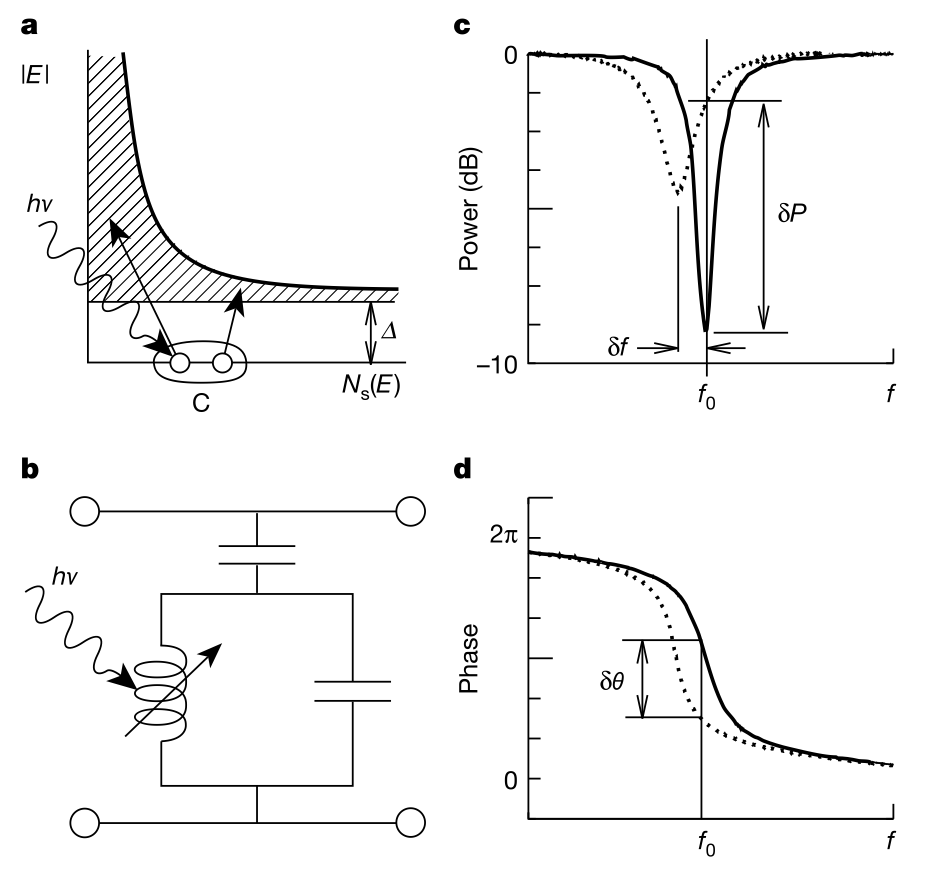
\includegraphics[width=0.55\columnwidth]{Schermata 2021-06-08 alle 13.47.58.png}
        \caption{
                \label{fig:pric} An illustration of the detection principle.
        }
\end{figure}
As we have already pointed out, KIDs can detect incoming particles through the properties of a LC superconducting circuit but now we can describe their working principle in a deeper way.\\
KIDs are biased with AC current so Cooper pairs are oscillating: this oscillation guarantees a certain amount of kinetic inductance.
When a particle or a phonon arrives, it is absorbed by the superconducting film ($T \ll T_C$) where it breaks Cooper pairs creating a number of quasi-particle excitations (Fig \ref{fig:pric}.a). This build up of quasi-particle density causes an increase of kinetic inductance. In order to measure quantitatively this effect we coupled the superconductive with a capacitor realizing a LC circuit (Fig \ref{fig:pric}.b). This acts like a resonator with a resonance frequency 
\begin{equation}
f_0 = \frac{1}{2 \pi \sqrt{LC}}
\end{equation}
($L \equiv L_{tot}$) and a high quality factor Q (order of $10^4$-$10^5$). Therefore a change in the internal inductance will modify the condition of the resonator leading to a new resonant frequency. The resulting fractional change in the resonance frequency $f_0$ is expressed as:
\begin{equation}
    \frac{\mid \delta f \mid}{f_0} = 0.5 \alpha \frac{\delta L_{tot}}{L_{tot}}
\end{equation}
where $\alpha$ represents the fraction of the total inductance of the transmission line that is contributed by the kinetic inductance:
\begin{equation}
    \alpha = \frac{L_{k}}{L_{tot}}
\end{equation}
Actually the effect of the incoming particle is twofold: the quasi-particles increase both the inductance and the resistance of the surface, which moves the resonance to a lower frequency (due to $L$) and makes the dip broader and shallower (due to $R$) (Fig \ref{fig:pric}.c). Both of these effects also contribute to changing the phase of a microwave probe signal transmitted though the circuit (Fig \ref{fig:pric}.d). As a result, it is possible to infer the energy that was deposited by monitoring the changes in the resonance parameters (the amplitude and the phase).\\
\begin{figure}[H] 
        \centering 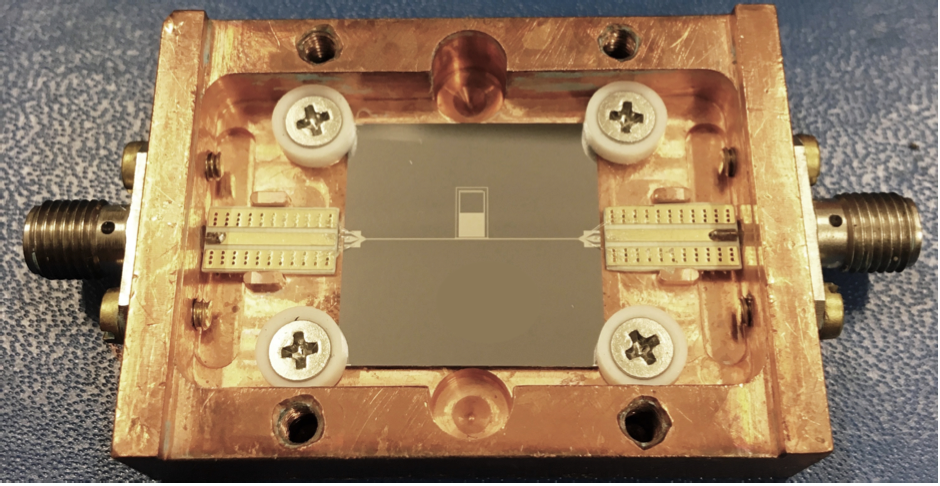
\includegraphics[width=0.9\columnwidth]{KID.png}
        \caption{
                \label{fig:KID} A single KID deposited on a 2 × 2 $cm^2$ Si substrate.
        }
\end{figure}

The main limitation of KIDs is the restricted active area (Fig \ref{fig:KID}), so it was added an indirect detection system in order to overcome this issue: the single KID is deposited on a large insulating substrate (Si) that mediates the particle interactions converting them into athermal phonons. The phonons that are not thermalized or lost through the substrate supports, reach the superconductor and break Cooper pairs, giving rise to the signal. This procedure is known as phonon-mediated approach and it guarantees an active area of the order of several $cm^2$ instead of few $mm^2$.
\section{Experimental setup}
Our task was to design and implement a readout for a single KID and to take and analyze some data coming from it.\\
However, before describing our work, it is important to go into further detail in the explanation of the cryogenic apparatus which contains the KID.
\subsection{Cryostat}
As we have already pointed out, KIDs are based on superconducting materials so we need cooling devices to temperatures around $10 \%$ of their superconducting transition temperature, $T_c$. Since our KID architecture is based on an aluminium resonator, we can reach the required range with a wet \ce{^{3}_{}He}/\ce{^{4}_{}He} dilution refrigerator with a base temperature of $10~mK$ and radiative shields at $600~mK$ and $4.2~K$ (Fig. \ref{fig:Cryo}). \\
\begin{wrapfigure}{l}{0.49\textwidth}
\centering
\vspace{-0.4cm}
    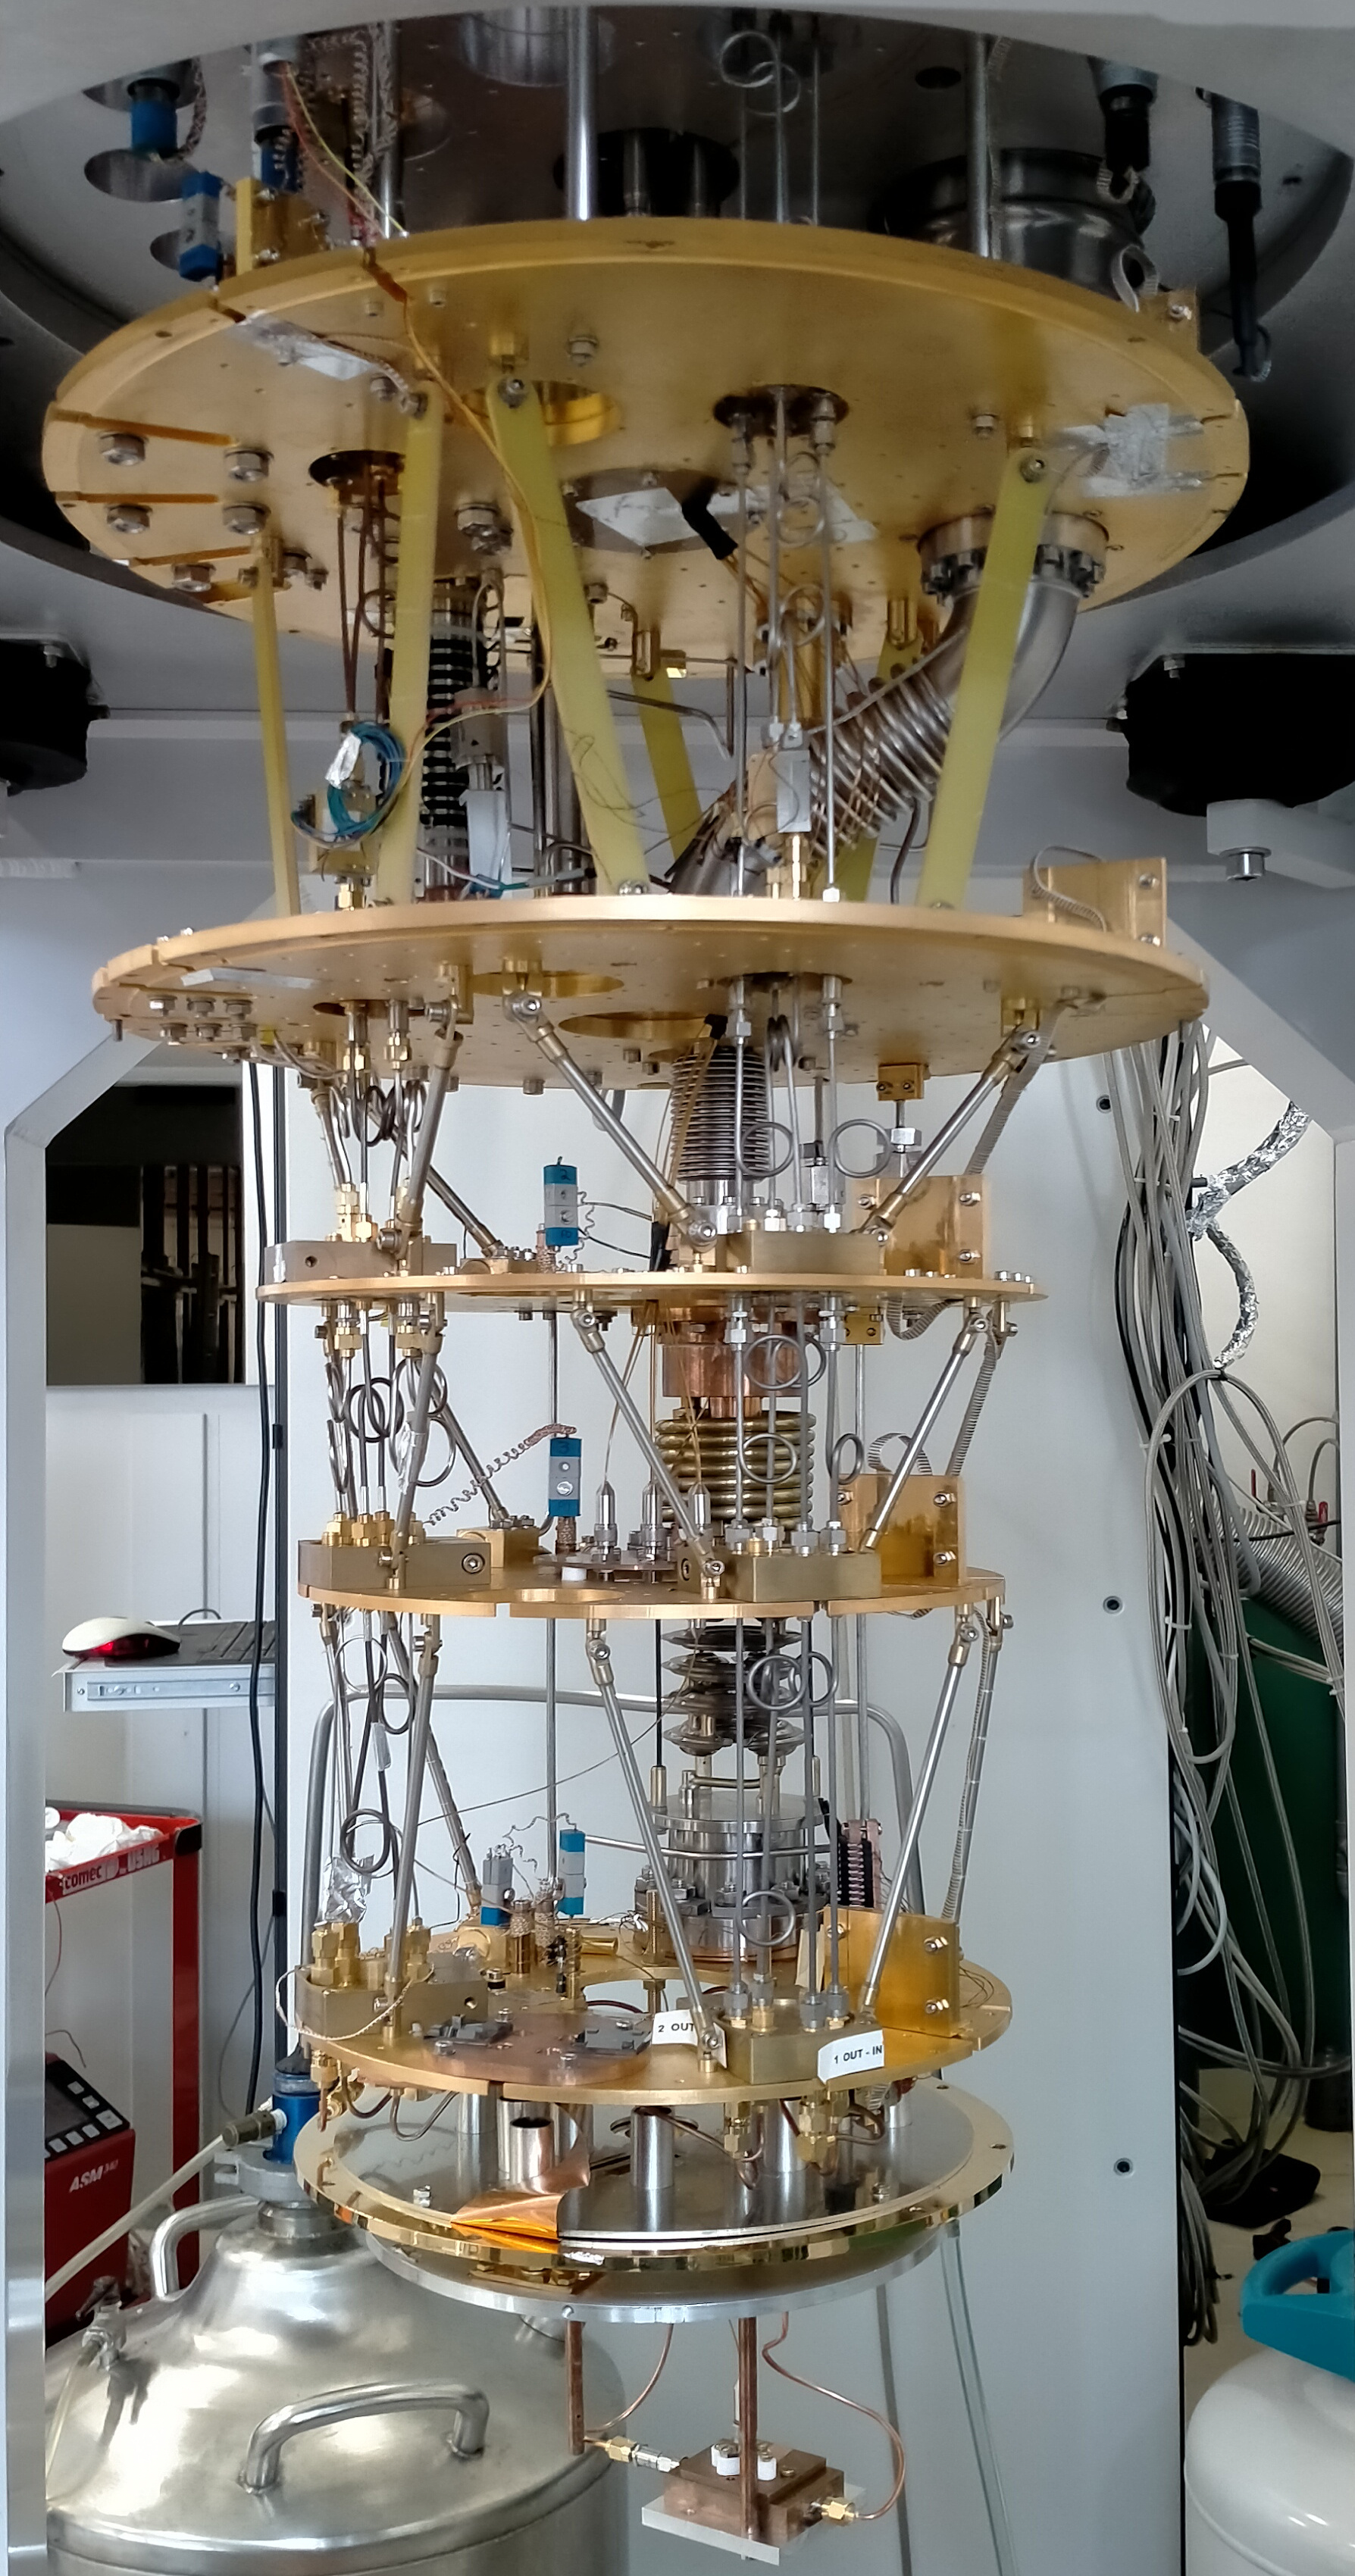
\includegraphics[width=0.43\textwidth]{IMG20210609095242.jpg}
  \caption{\label{fig:Cryo} Cryostat setup.}
\end{wrapfigure}
In order to construct a refrigerator based on the dilution process, it is necessary to accomplish two primary objectives: first, a mixture of \ce{^{3}_{}He}/\ce{^{4}_{}He} in the correct proportions must be allowed to condense and undergo a phase separation and secondly, the \ce{^{3}_{}He} must be preferentially recycled from the dilute phase (that is \ce{^{4}_{}He}-rich phase), recondensed, and then returned to the concentrated phase (that is \ce{^{3}_{}He}-rich phase). For what concerns the correct proportions, the dilute phase contains about $6.6 \%$ \ce{^{3}_{}He} and $93.4 \%$ \ce{^{4}_{}He}. Regarding the \ce{^{3}_{}He} cycle instead, it start
s when the isotope enters the cryostat at a pressure of a few hundred millibar (reached with the help of vacuum pumps at room temperature) and it is precooled and purified by liquid nitrogen at $77~K$ and then cooled by a \ce{^{4}_{}He} bath at $4.2~K$. Then, thanks to a $1~K$ bath, the \ce{^{3}_{}He} is further cooled up to $1.2-1.5~K$ in a vacuum chamber. As the pressure of the \ce{^{3}_{}He} is greater than its vapor pressure, the $1~K$ bath liquifies it and removes the produced condensation heat. Next, the isotope flow exchanges heat with the still at a temperature which is around $0.5$ to $0.7~K$ and then it is further cooled down in a set of counterflow heat exchangers by a cold flow of \ce{^{3}_{}He} moving in the opposite direction. Finally, the pure \ce{^{3}_{}He} enters the mixing chamber where the \ce{^{3}_{}He}/\ce{^{4}_{}He} mixture is kept at a temperature that allows to maintain two separate phases, one \ce{^{3}_{}He}-rich phase floating on top and the other \ce{^{4}_{}He}-rich heavier phase downward. If we remove \ce{^{3}_{}He} from the diluted phase, \ce{^{3}_{}He} atoms from the concentrated phase will cross the phase boundary to occupy the vacant energy states. This process is called dilution and the heat it needs to happen is the cooling power of the refrigerator.\\
For what concerns the cold electronics, the sensor, which works at $70~mK$, is followed by a low noise cold amplifier (LNA) operated at $4~K$. Due to the low temperature working conditions, the KID is at thermal contact with the coolest golden plate inside the cryostat. In addition, in order to protect the chip from external radiation and to guarantee a further thermal shield the system of golden plates is nested in many concentric screens (the external screen is visible in Fig. \ref{fig:Stanza}).
\begin{figure}[H]
\centering
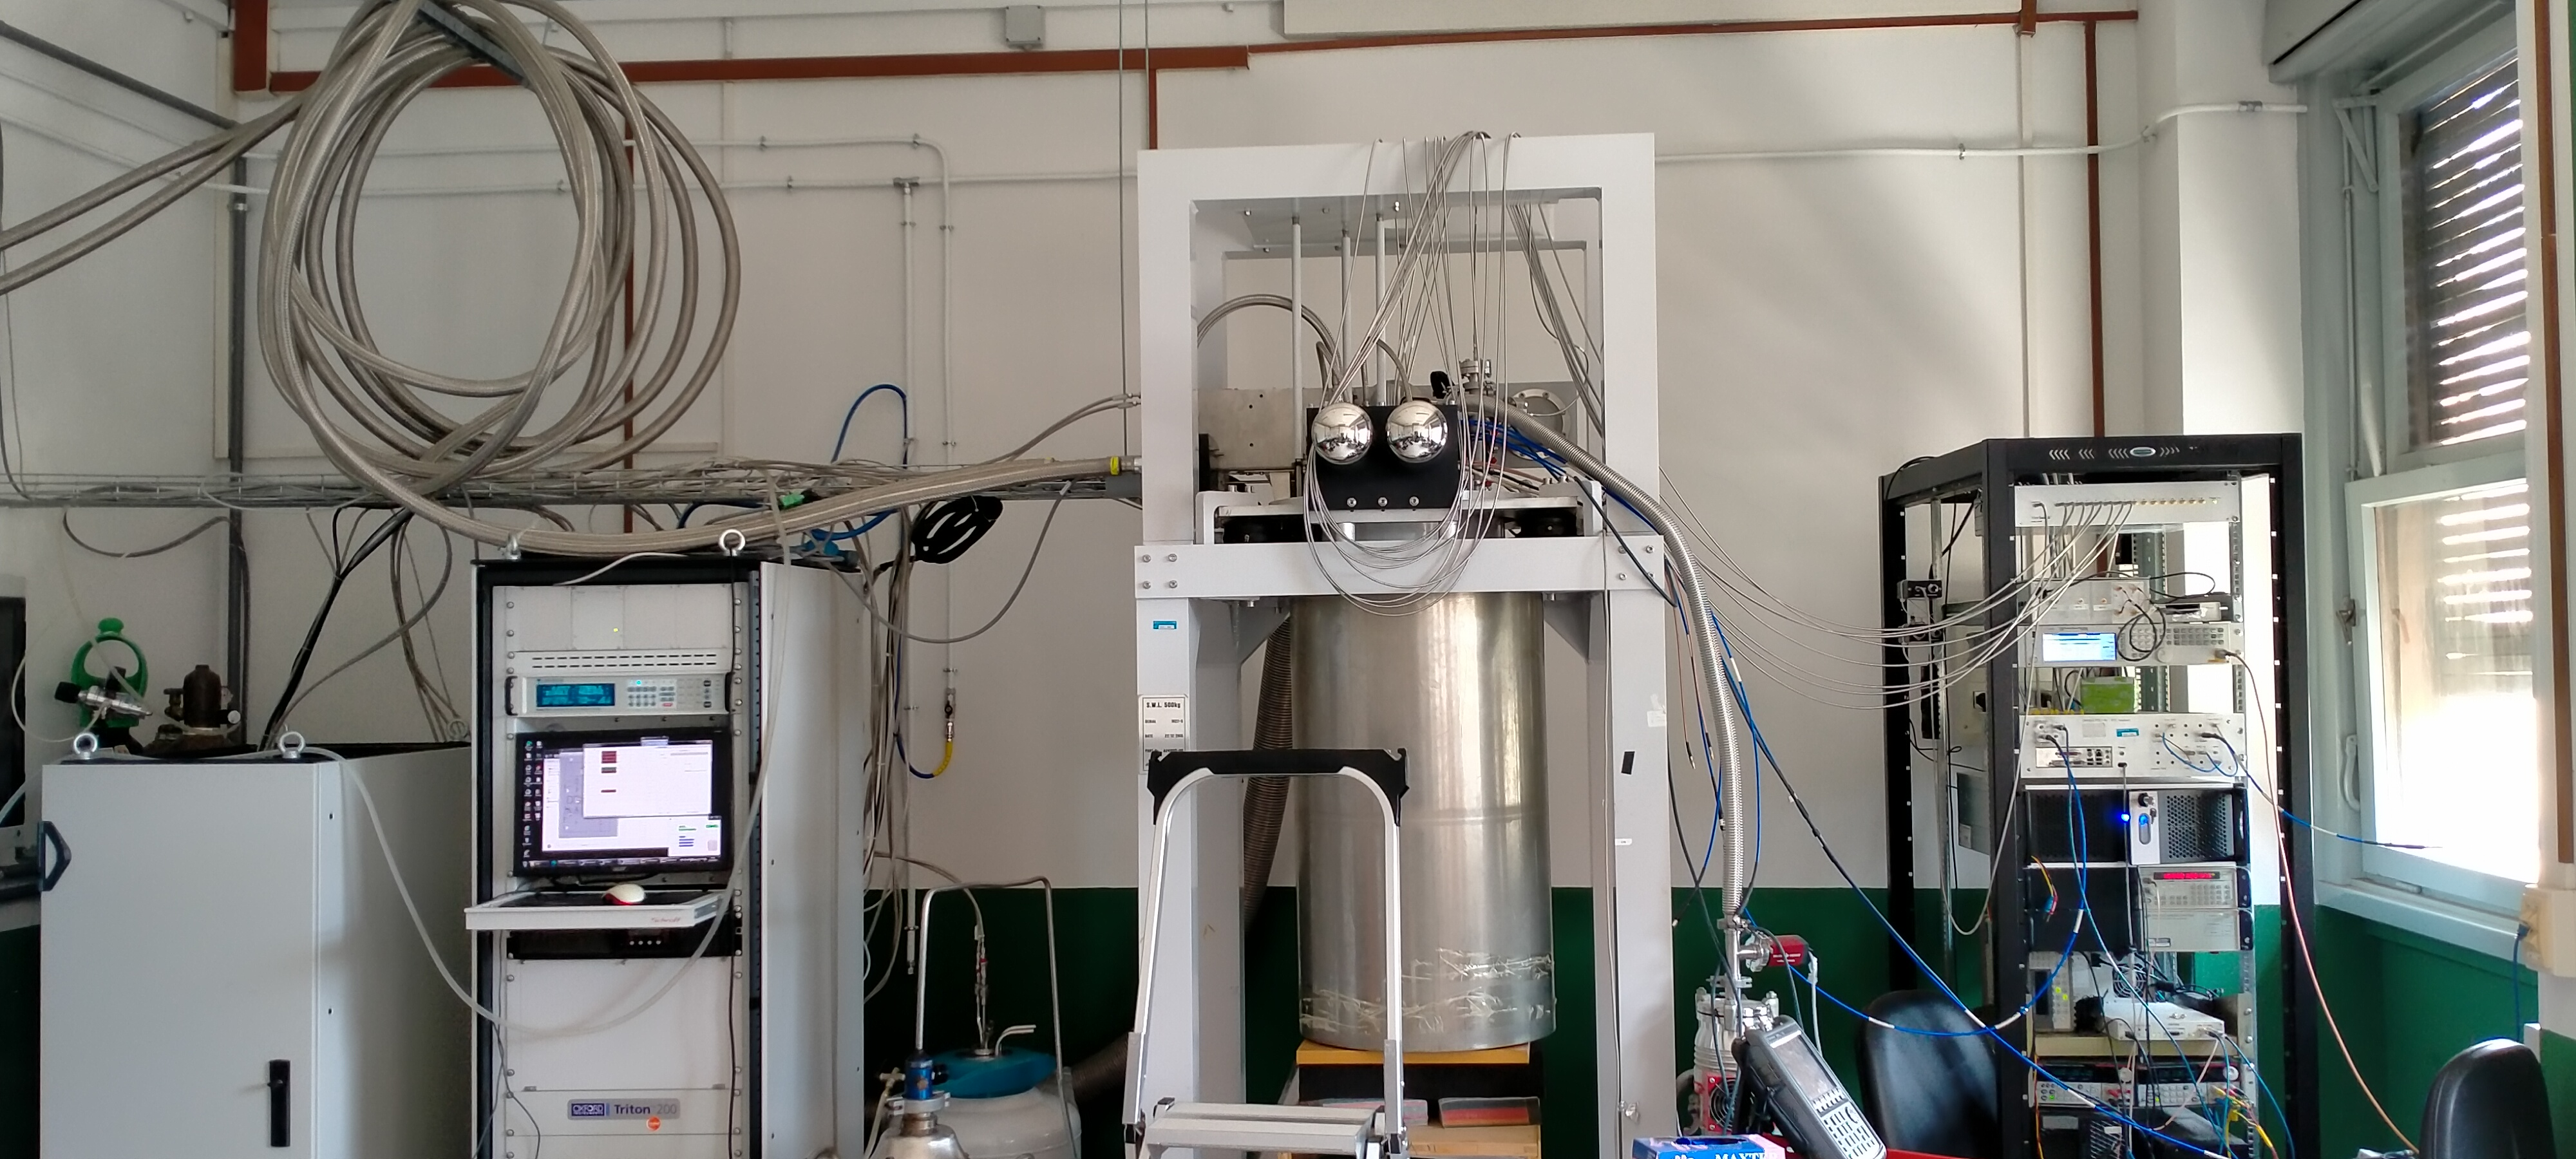
\includegraphics[width=0.9\textwidth]{stanza.jpg}
\caption{\label{fig:Stanza} A view of the cryostat from outside.}
\end{figure}
\subsection{Readout concept}
Our readout was based on the so-called homodyne detection, which is based on the comparison of a RF signal, carrying some low frequency information on top of a particular RF sinusoidal signal (the so called Local Oscillator) with respect to the Local Oscillator itself.
In other words, the readout consists in extracting the baseband frequency signal from the RF signal, by simply subtracting in frequency the RF signal from the LO one, similarly to what happens with the frequency modulation radio. This frequency subtraction is achieved using a non-linear circuit element such as the IQ mixer, which outputs the I (in-phase) and Q (quadrature) components of the signal, corresponding to its real and imaginary part. These two channels, at baseband frequency, are then easily sampled by an Arduino Due microcontroller. Next, the signal phase is reconstructed and the height of the phase pulses, proportional to the energy absorbed by the resonator, is finally analyzed.\\
Our design of the readout consists in three sections: an RF and a baseband circuit (mounted on a prototype breadboard), followed by a two-channel digitizer, that is the ADC of an Arduino DUE. The microcontroller is capable of sampling at about 333 kHz, but it is limited to 206 kHz in the real data-taking in order to be able to also act as an online trigger.
\begin{figure}[H]
        \centering
        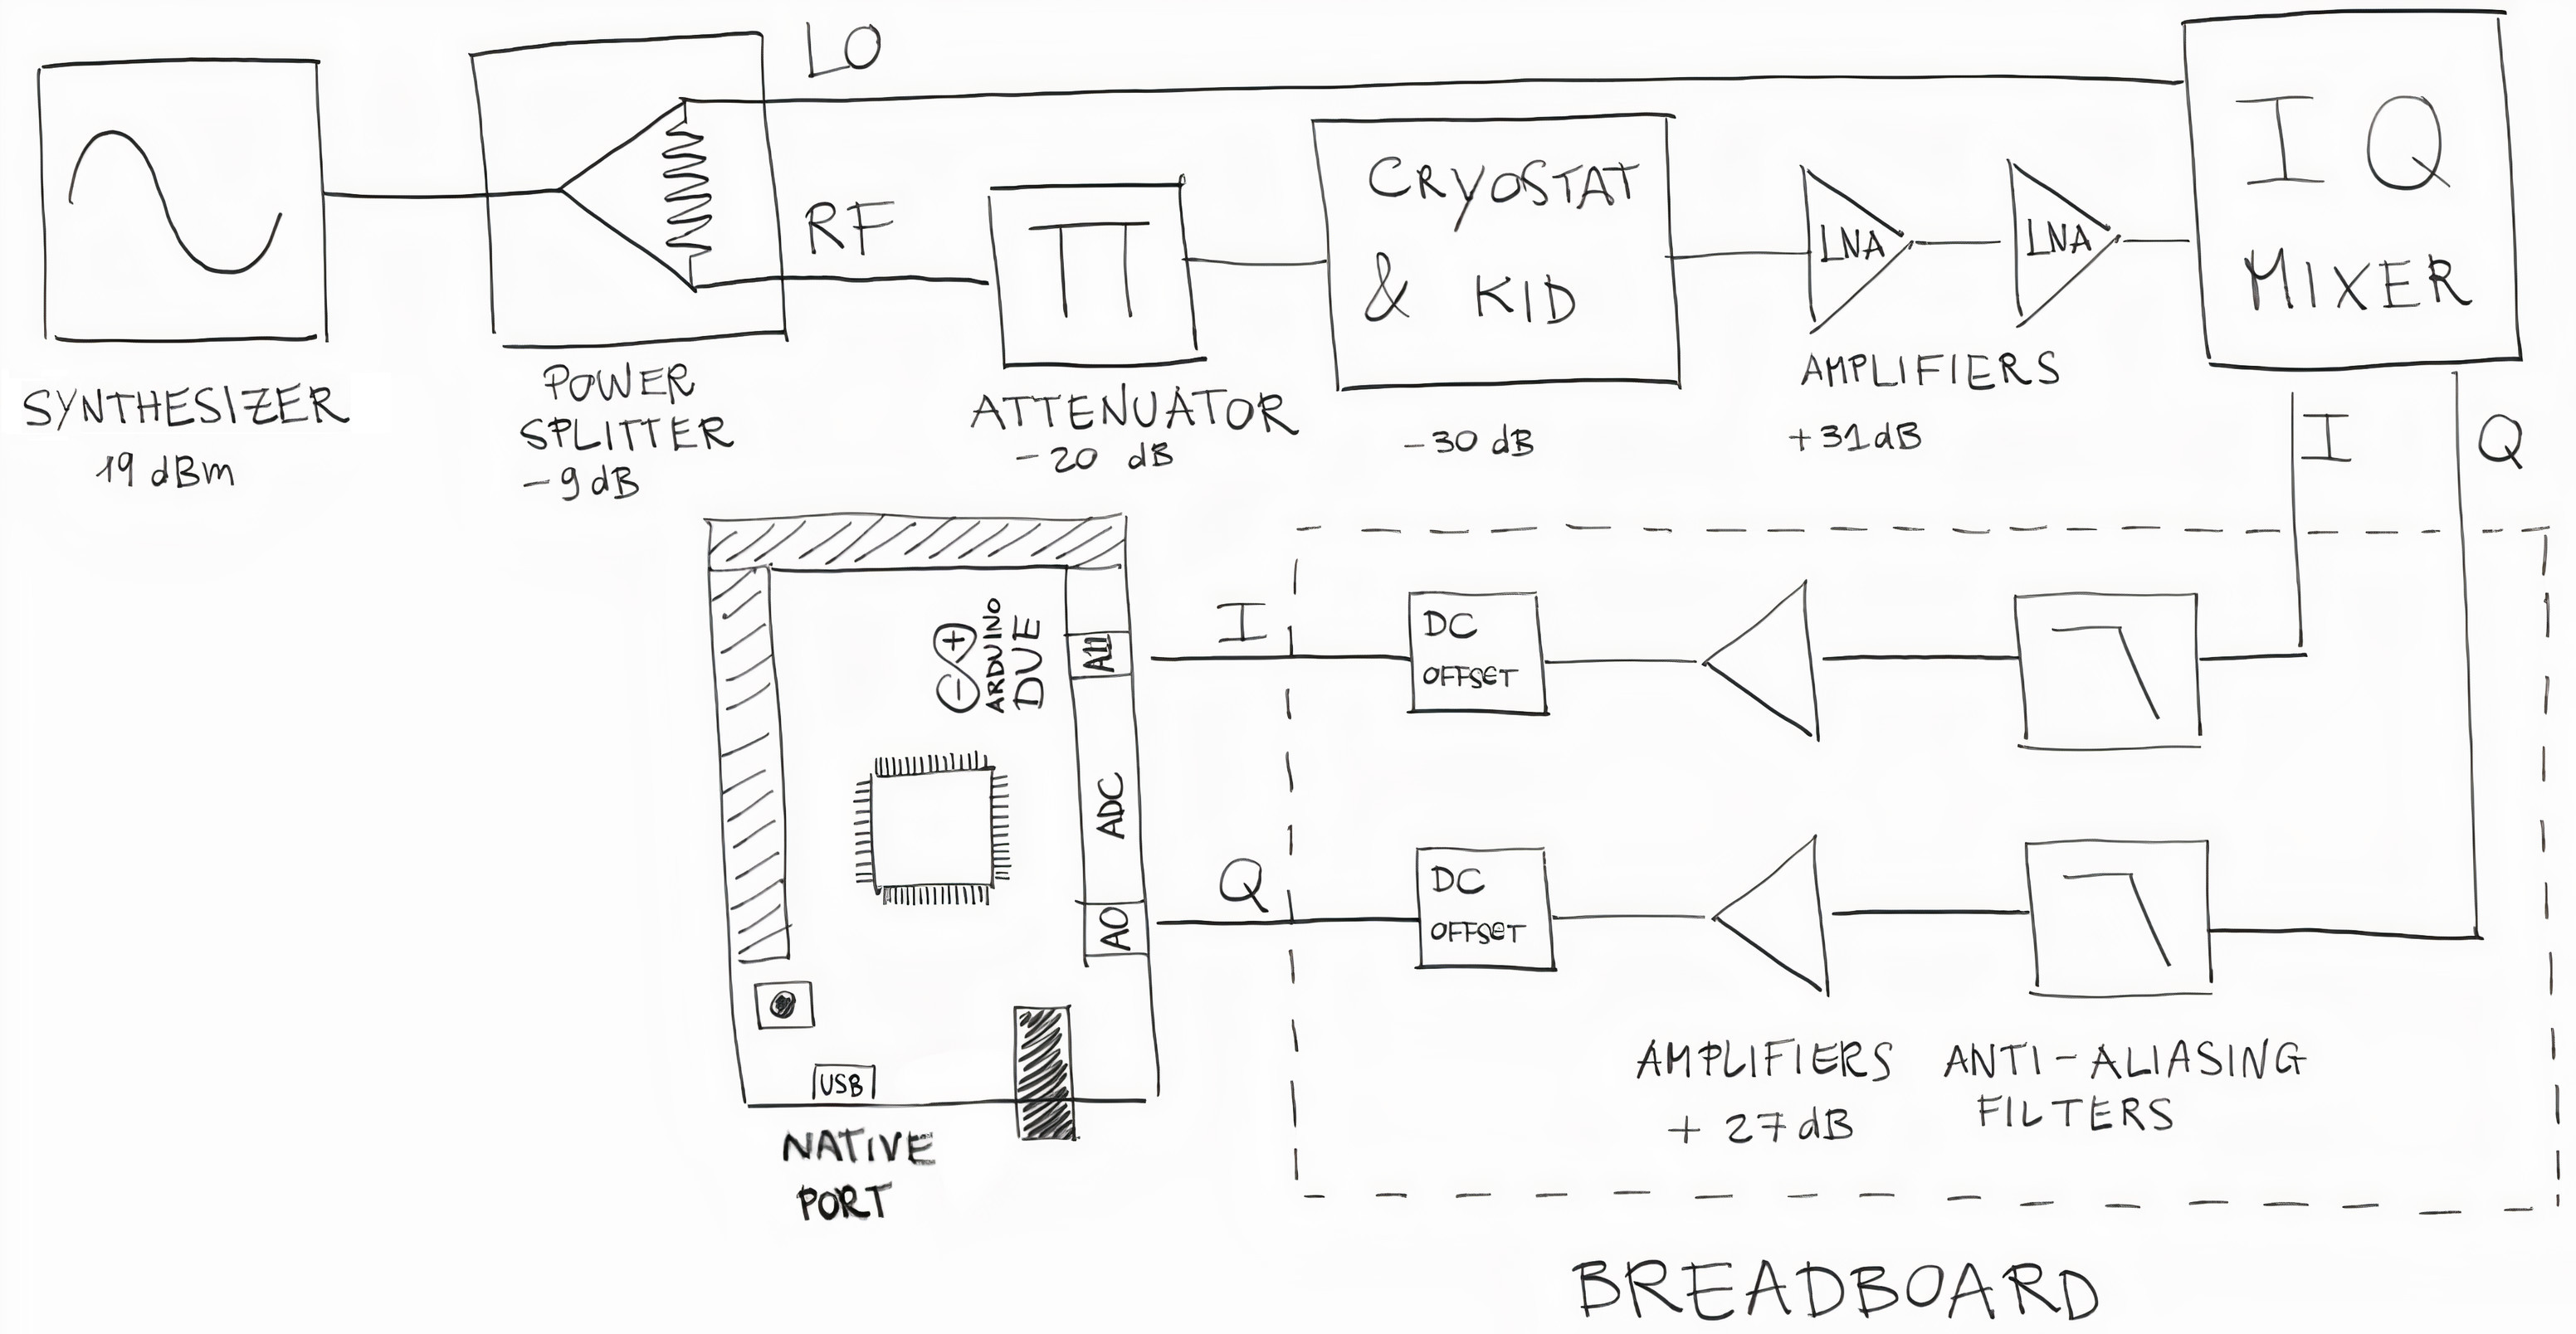
\includegraphics[width=\textwidth]{schema.jpg}
        \caption{Homodyne Readout schematic.}
        \label{scheme}
    \end{figure}
\begin{figure}[H]
\centering
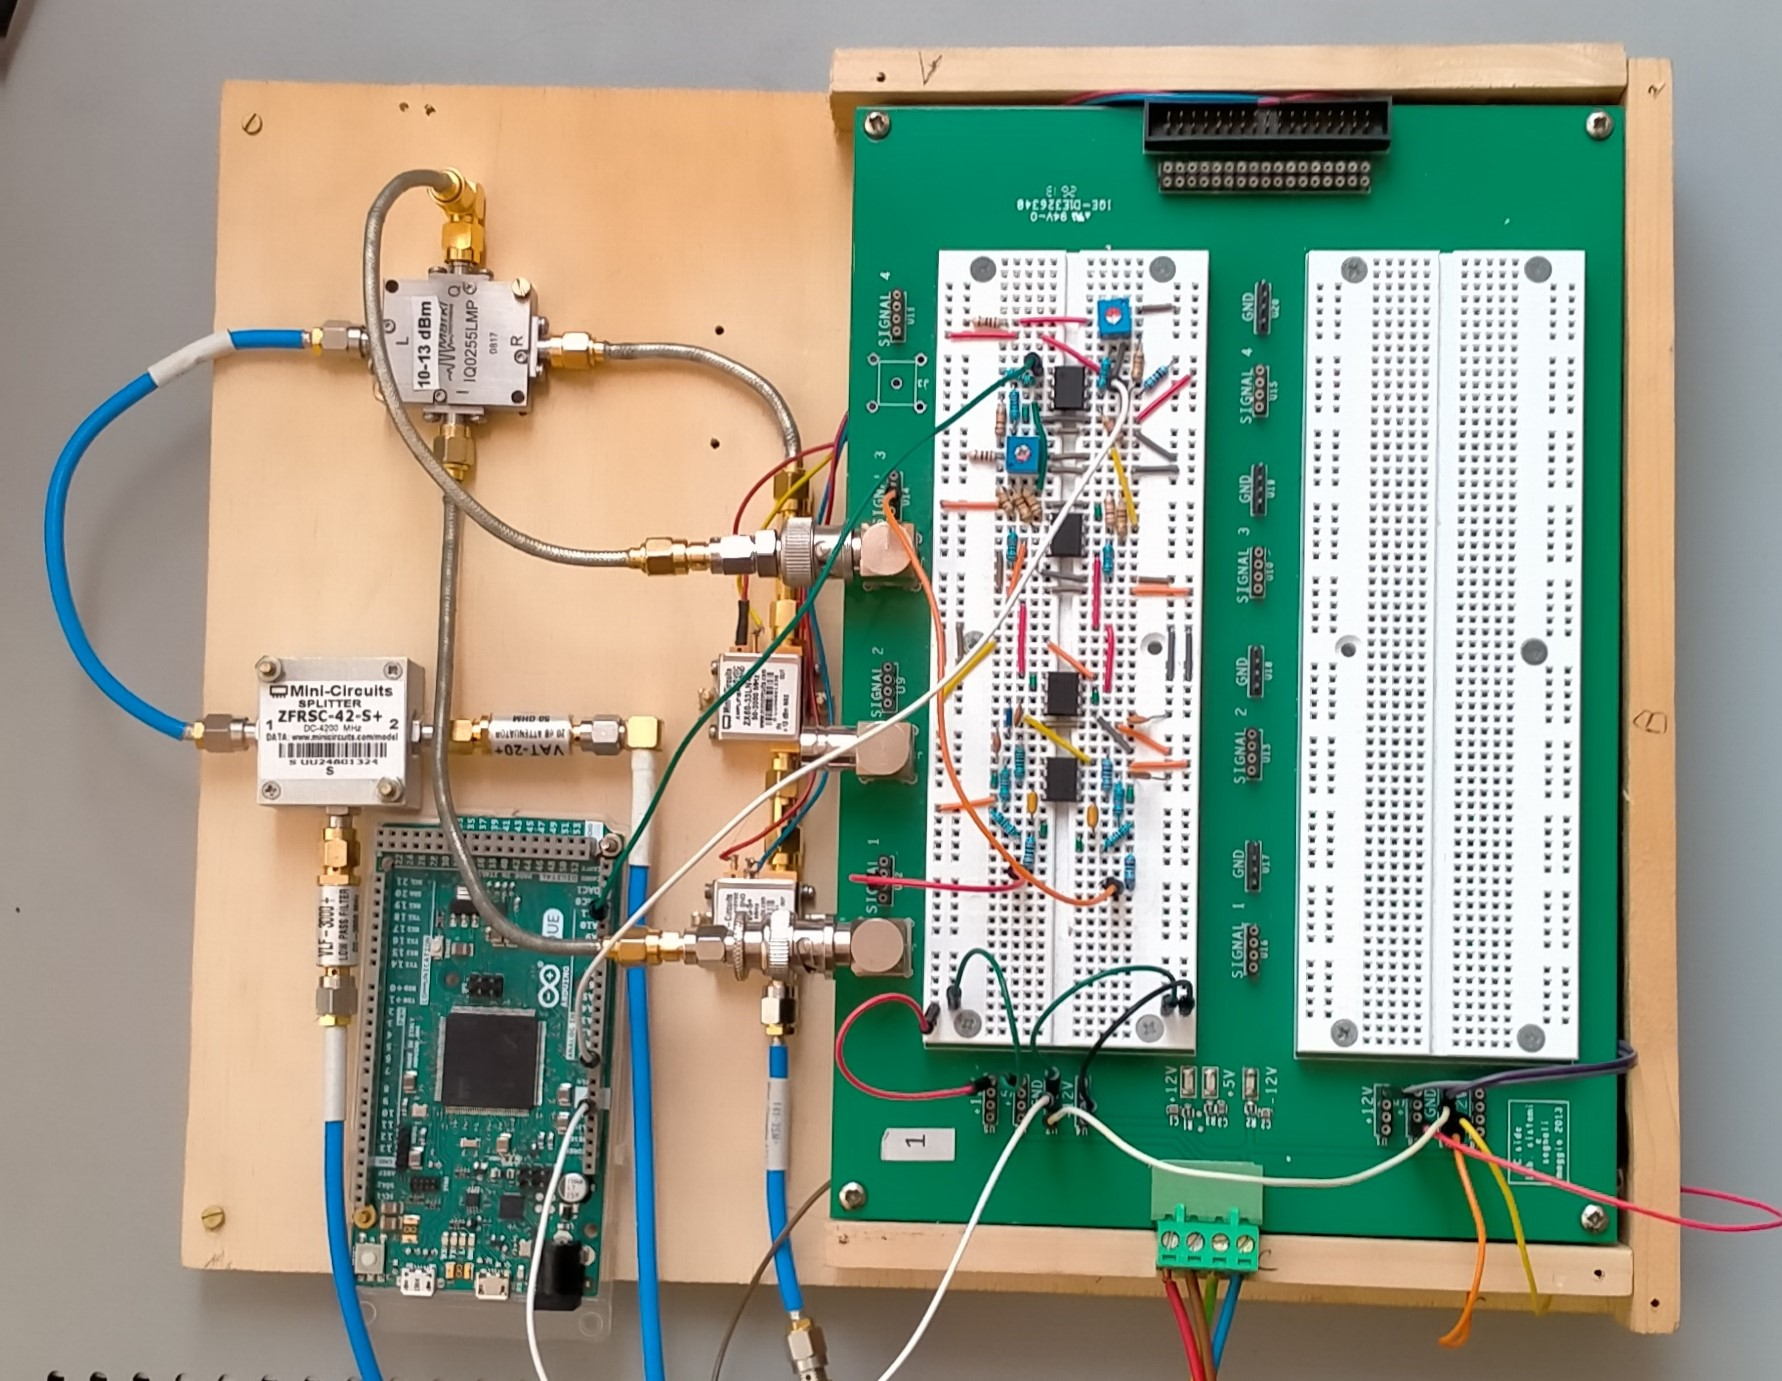
\includegraphics[width=0.58\textwidth]{circuitocompleto.jpg}
\caption{Complete readout system picture. Before the data-taking, several flexible jumpers were replaced with rigid ones (not shown in figure) to reduce the noise generated by vibrations.}
\end{figure}
\subsection{Radio frequency circuit}
A radio frequency synthesizer (Agilent MXG Analog Signal Generator N5182B) generates the LO cosine signal, which is divided by a power splitter into two copies with a 9dB loss. One of the two channels goes into the LO port of an IQ mixer, while the other one is attenuated by 20dB before entering the cryostat (in order to match the correct working point of the resonator), passes through the KID resonator and then goes through a 40dB CITLF3 SiGe cryogenic low noise amplifier.
The whole cryostat provides an attenuation of about 30dB to the baseline, in addition to the stopband effect of the resonator.
Outside the cryostat, at room temperature, the RF signal is amplified by 31 dB by a couple of cascade low-noise amplifiers, and then goes in the RF port of the IQ mixer.
\begin{figure}[H]
        \centering
        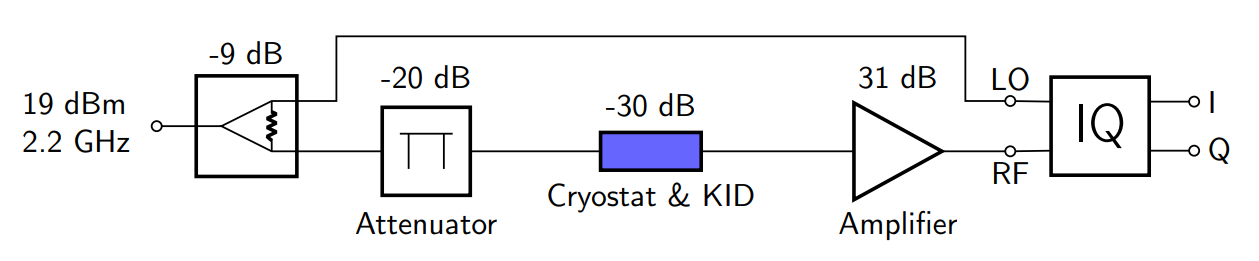
\includegraphics[width=\textwidth]{RFcircuito.PNG}
        \footnotesize{\caption{RF circuit schematic. Note that the RF amplitude, measured at the mixer input, is $V_p = -8.791(3)$ dBm, corresponding to a $V_{pp} \sim 230 mV$}}
        \label{RFcircuit}
    \end{figure}
\subsubsection{IQ mixer}
The IQ mixer is a Marki Microwave IQ0255LMP and consists of two identical down-conversion mixers where the RF ports are connected with an in-phase power splitter and the LO ports are connected with a quadrature hybrid, a special power splitter that also creates a $90^\circ$ phase shift between the two outputs.\\
The output of a normal mixer, unlike an IQ one, is the product of the two inputs. By expoiting the trigonometric Werner formulas, indeed, we know that:
\begin{equation}
A(t) = \cos \omega_1 t, \, B = \cos \omega_2 t \Rightarrow A(t) B(t) = \frac{1}{2} \left[ \cos (\omega_1 + \omega_2) t + \cos (\omega_1 - \omega_2) t\right]
\end{equation}
In the down-conversion mixer, we only obtain a signal at a frequency which is the difference of the LO and RF frequencies, because the $\cos (\omega_1 + \omega_2) t$ component is suppressed.
\begin{figure}[H]
        \centering
        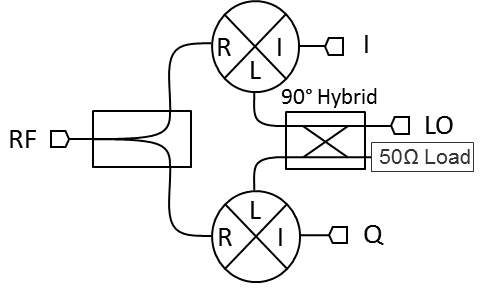
\includegraphics[width=0.5\textwidth]{iqmixer.png}
        \caption{IQ mixer scheme}
        \label{IQmix}
    \end{figure}
More specifically, if:
\begin{equation}
LO(t) = a_{LO}\sin(\omega_{LO}t), \, RF(t) = a_{RF}\sin(\omega_{LO}t + \phi)
\end{equation}
where the $a_{RF}$ and $\phi$ also depend on time but at a much lower frequency (e.g. kHz) with respect to $\omega_{LO}$ (e.g. GHz).
then:
\begin{align}
& LO(t) \cdot RF(t) = a_{LO}a_{RF}\sin(\omega_{LO}t)\sin(\omega_{RF}t + \phi)\\
&= \frac{a_{LO}a_{RF}}{2} \Big( \cos((\omega_{RF}-\omega_{LO})t + \phi) - \cos((\omega_{RF} + \omega_{LO}) t + \phi) \Big)
\end{align}
and:
\begin{align}
& LO(t+\frac{\pi}{2})\cdot RF = a_{LO}a_{RF}\cos(\omega_{LO}t)\sin(\omega_{RF}t + \phi)\\
&= \frac{a_{LO}a_{RF}}{2} \Big( \sin((\omega_{RF}-\omega_{LO})t + \phi) + \sin((\omega_{RF}+\omega_{LO}) t  + \phi) \Big)
\end{align}
For $\omega_{LO} = \omega_{RF}$ and suppressing the $2\omega_{LO}$ components, we can define:
\begin{align}
I = \frac{LO(t) \cdot RF(t) }{\Lambda_I} &= \frac{a_{LO}a_{RF}}{2 \Lambda_I}\cos(\phi) \\
Q = \frac{LO(t+\frac{\pi}{2}) \cdot RF(t)}{\Lambda_I} &= \frac{a_{LO}a_{RF}}{ 2 \Lambda_Q}\sin(\phi)
\end{align}
where the two $\Lambda$s are dimensional constants.\\
In other words, for an ideal IQ mixer the outputs are the real part, in the I (in-phase) channel, and the imaginary part, in the Q (quadrature) channel, of the baseband frequency signal.\\
Note that both $a_{RF}$ and $\phi$ (amplitude and phase of the RF signal) are functions of frequency because of non-linear effects and the finite speed of the signal ($\sim 0.7c$), which implies that the same transmission line phase-shifts the signal differently at different frequencies. Moreover, the IQ mixer is a real object, therefore the ideal behaviour is valid only in some range of frequencies (1.5 - 4.5 GHz in our case).\\
For these reasons, an initial calibration is needed to evaluate the offsets, the amplitudes and the conversion losses for the two channels of the mixer. These parameters will be needed in the choice of the elements in the baseband frequency circuit, which is essential in order to exploit the complete dynamical range (0-3.3V) of the ADC.\\
The calibration was made by introducing different phase-shifts in the RF signal with a 4m long coaxial cable as transmission line, while operating a frequency sweep in the range 2.180-2.217 GHz through the RF generator, which output a cosine signal with an amplitude of 19 dBm. A Keysight FieldFox RF Vector Network Analizer was used for diagnostics during the circuit construction.
We also attenuated the signal by 30 dB to simulate the presence of the cryostat. The RF amplitude, measured at the mixer input with the VNA, is equal to -8.791(3) dBm, corresponding to 115 mV.\\
The I and Q channels were read using a Keysight DSOX1204G oscilloscope (also used in all the other cases) and visualized in the I-Q plane, as shown in figure.
\begin{figure}[H]
        \centering
        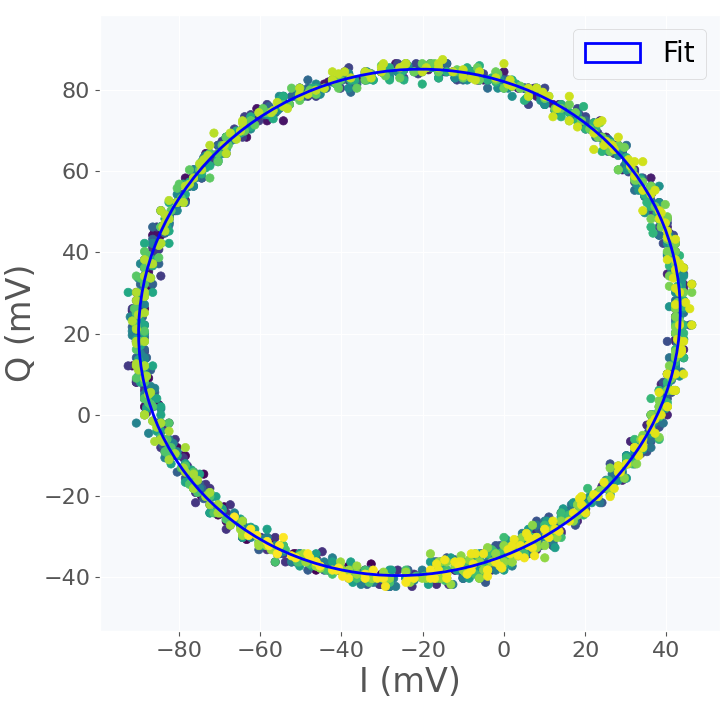
\includegraphics[width=0.5\textwidth]{oscilloscope_circle_before_if_circuit.png}
        \caption{I and Q scatter plot and ellipse fit, using the formula $ \left(\frac{I - I_c}{I_a} \right)^2 + \left(\frac{Q - Q_c}{Q_a} \right)^2 = 1 $}
        \label{IQfit}
    \end{figure}
Theoretically the resulting curve should be a circle, but the mixer has different conversion losses for I and Q, so the data was fitted with a slightly eccentric ellipse, with parameters $I_c = -23.255(3)$ mV,\, $Q_c = 22.267(3)$ mV, $I_{a} = 67.009(2)$ mV and $Q_{a}= 61.908(2)$ mV.
\subsection{Baseband circuit}
Since the goal was to sample with an Arduino Due, which has a dynamical range of 0-3.3 V, it was necessary to design a baseband circuit in order to both maximize the dynamics of the signal and to make sure that all the sampled points fell in the (0-3.3V) square in the IQ plane. The circuit was implemented in two copies, one for each channel, and mounted on a single prototype breadboard.
\begin{figure}[H].
        \centering
        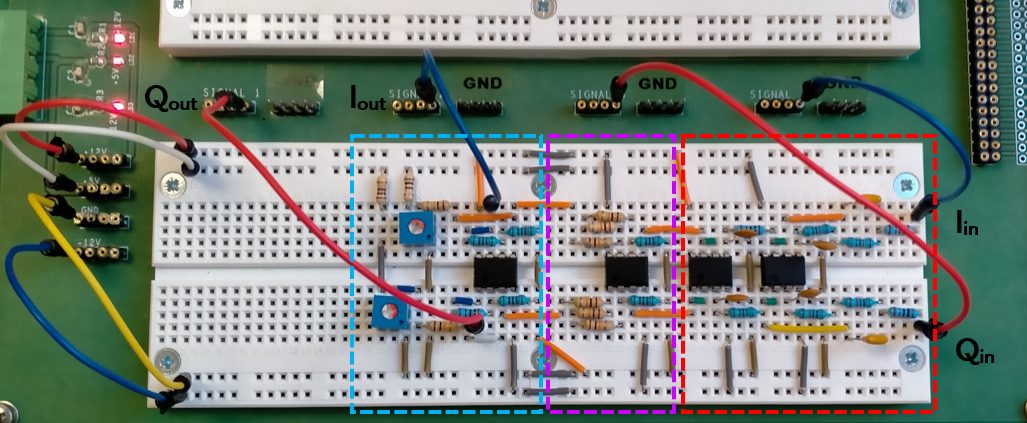
\includegraphics[width=0.80\textwidth]{circuitobase.PNG}
        \caption{Complete baseband circuit view: the I channel is processed in the upper half of the breadboard and the Q channel in the lower one. The colored boxes are: \textcolor{red}{anti-aliasing filters}, \textcolor{violet}{amplifiers} and \textcolor{cyan}{summing circuits} }
        \label{breadboard}
    \end{figure}
\subsubsection{Anti-aliasing filter}
First of all, the signal passes through a 3rd order anti-alias Bessel filter. Considering that the pulses generated by the resonator during the absorption of the energy from particles have characteristic frequencies up to 40 kHz and Arduino's sampling rate is around 330 kHz, the passband (-3dB) and stopband (-20dB) frequencies were respectively set to 50 kHz and 160 kHz. In the real data-taking, when the ADC works at 206 kHz, the filter response is -17 dB at the Nyquist frequency, so we consider it still sufficient to suppress the aliases.
    \begin{figure}[H]
        \centering
        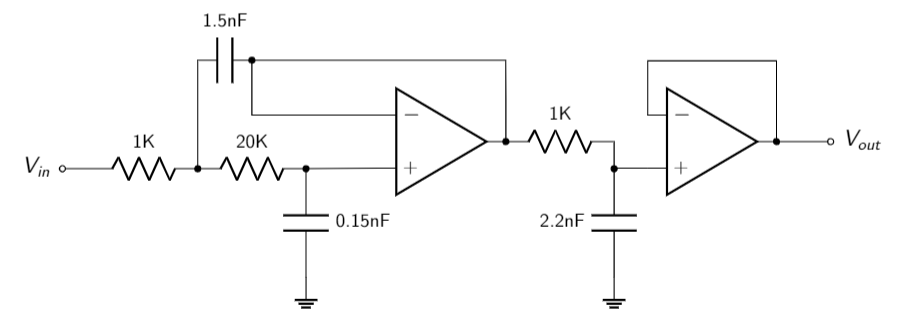
\includegraphics[width=0.8\textwidth]{bessel.PNG}
        \caption{Bessel circuit schematic, the filter is composed by two stages: a 2nd order Sallen-Key and a 1st order buffered RC. The op-amp used is a TL-082.}
        \label{bessel}
    \end{figure}
The type of filter designed permitted to achieve a roll-off of 60 dB/Decade (estimated knowing that the response is -11dB at 100kHz and -40dB at 300 kHz), as expected for a 3rd order filter, and a maximally flat group delay.
After building the filters, the requirements were verified with the oscilloscope using the frequency response function. The measured passband and stopband frequencies are $49.6(1)$ kHz and $145.9(1)$ kHz for the I channel and $52.4(1)$ kHz and $153.0(1)$ kHz for the Q channel. The flatness of the group delay, i.e. the linearity of the phase response has been checked through a linear fit in the signal band.
\begin{figure}[H]
    \centering
    \begin{subfigure}{0.52\textwidth}
    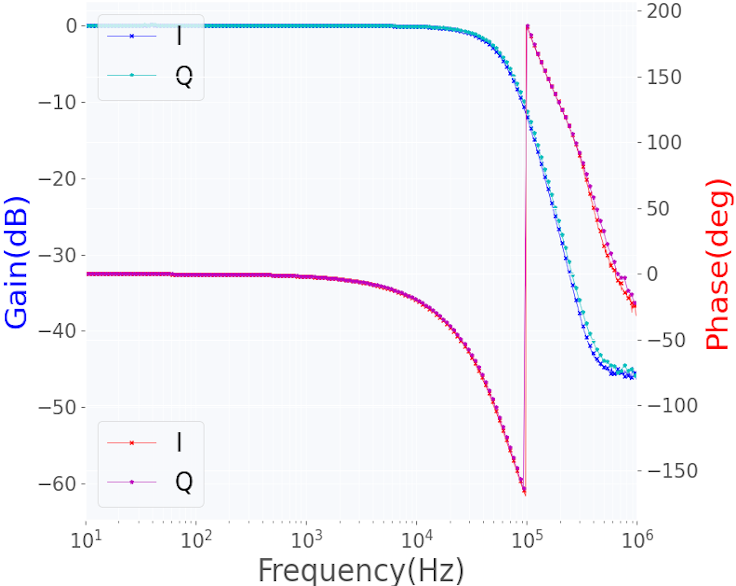
\includegraphics[width=\textwidth]{besselbest.png}
    \caption{Gain and phase responses.}
    \end{subfigure}
    \begin{subfigure}{0.47\textwidth}
     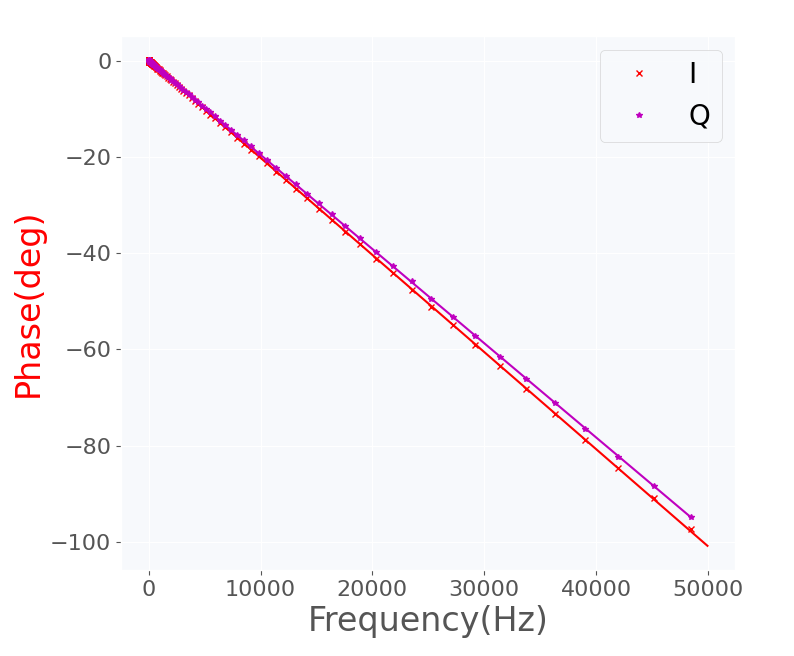
\includegraphics[width=\textwidth]{fitbessel.png}
           \caption{Phase response linear fit up to 50 kHz.}
    \end{subfigure}
    \end{figure}

\subsubsection{Amplifier and Summing Circuit}
We also developed a simple non-inverting amplifier with a gain of 27dB, followed by a summer circuit (a non-inverting amplifier with a gain of 1) to maximize the signal range, starting from $Q_{pp} < I_{pp} < 160$ mV, while keeping the values contained in the ADC range of 0-3.3V. 
\begin{figure}[H]
\centering
\begin{subfigure}{0.48\textwidth}
\centering
        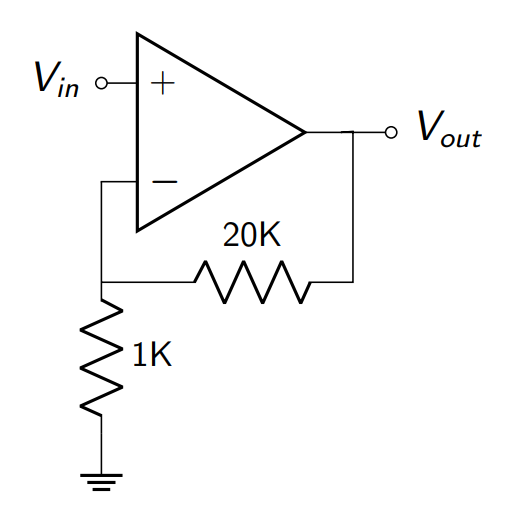
\includegraphics[width=0.7\textwidth]{amp.PNG}
        \caption{Non-inverting amplifier circuit diagram}
        \label{amp}
    \end{subfigure}
\begin{subfigure}{0.48\textwidth}
\centering
        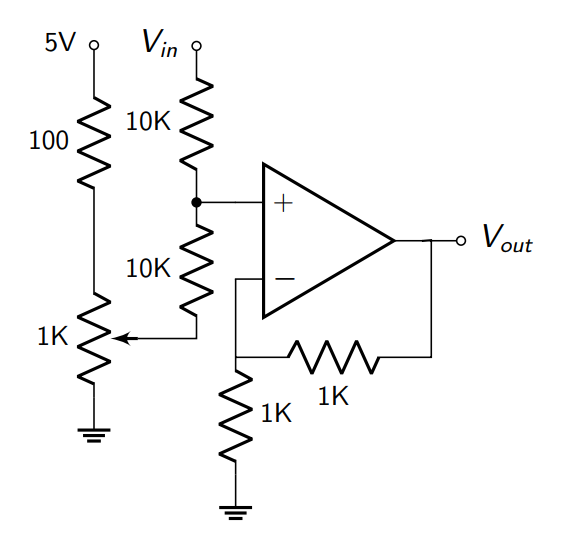
\includegraphics[width=0.73\textwidth]{summing.PNG}
        \caption{Summing circuit diagram}
        \label{summing}
        \end{subfigure}
    \end{figure}
The complete circuit response has been measured through the oscilloscope, as shown in figure, and the requirements have been successfully verified.
\begin{figure}[H]
    \centering
    \begin{subfigure}{0.49\textwidth}
    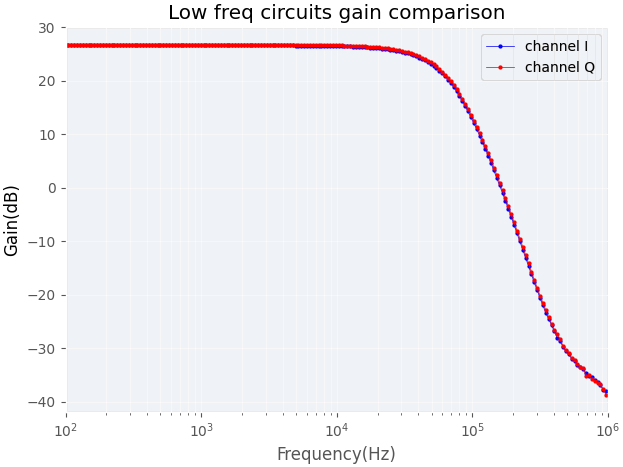
\includegraphics[width=\textwidth]{circuitgain.png}
    \caption{Gain response}
    \end{subfigure}
    \begin{subfigure}{0.49\textwidth}
     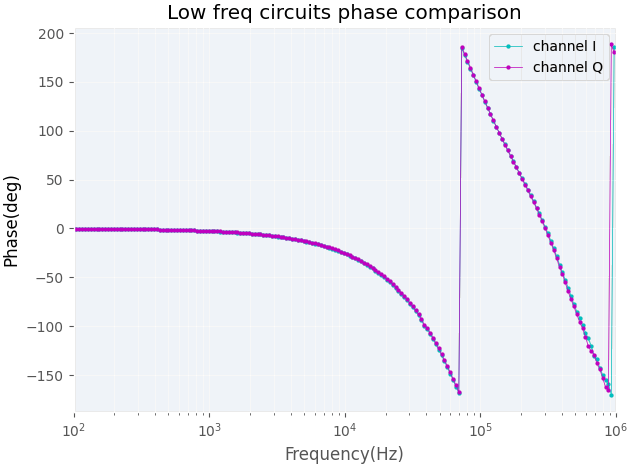
\includegraphics[width=\textwidth]{circuitphase.png}
           \caption{Phase response, modulo $\pm180^{\circ}$}
    \end{subfigure}
    \caption{Complete circuit responses}
    \end{figure}
\subsection{Data Acquisition}
\subsubsection{Digitizer}
Our DAQ hardware consists in an Arduino DUE connected to a laptop which runs a Python script. The microcontroller samples 2 analog channels via its internal 12 bit ADC. We set the ADC registers to the Free-Run mode, in which the conversions are continously performed (at the maximum speed allowed by the ADC clock) and an interrupt signal is called as soon as the digital value is available. This setting lets the sampling rate increase from 100 kHz (using the usual analogRead function) to 333 kHz.
\subsubsection{Online trigger}
In order to reduce the amount of data to transmit out of Arduino, an online trigger is needed. Our triggering algorithm consists in smoothing the waveforms through a moving average over a window of 10 samples and triggering with a threshold on the derivatives of I (calculated as $(I_n - I_{n-10})/10)$). Indeed, as Arduino floating point handling is quite slow, we preferred to apply the cut just as $(I_n - I_{n-10}) > \text{threshold}$. Note that the transmitted data are not smoothed, because offline we need the raw values to make a finer analysis.\\
The threshold is calculated at the beginning of the data taking, as 5.8 times the standard deviation of the derivative of the smoothed noise.
The value of 10 has been chosen because it is the number of points contained in the signal rise. On the other hand, the value of 5.8 has been chosen (through a simulation of the trigger on non-triggered data) to have a lowest false negative rate (nearly all the real signal gets triggered) and a low false positive rate (30\% of the triggered signal only contain noise). Afterwards, a more involved offline selection is applied.\\
Unfortunately, Arduino DUE's clock is rather slow (84 MHz), so the smoothing procedure slows down the data taking to 206 kHz, as shown in figure.
\begin{figure}[H]
\centering
    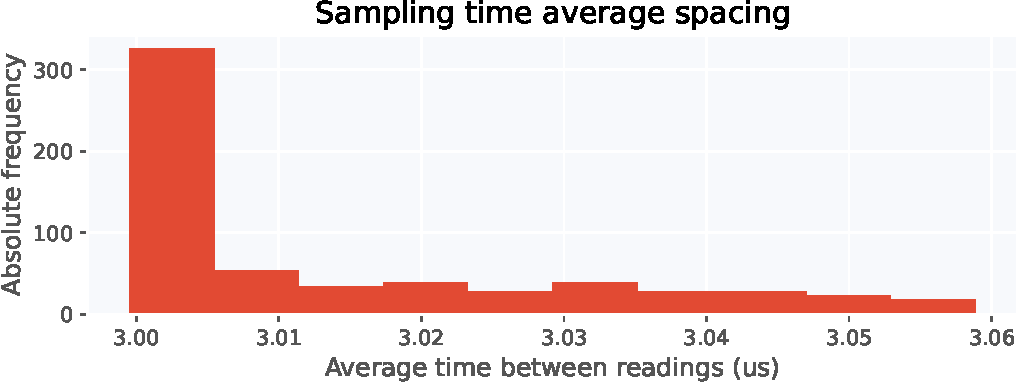
\includegraphics[width=0.65\textwidth]{samplingrate_orig.pdf}
    \caption{Sampling time average spacing ($\Delta T / N$) without smoothing for $\sim 600$ signals. It corresponds to a sampling rate of nearly 333 kHz.}
\end{figure}
\vspace{-0.4cm}
\begin{figure}[H]
\centering
    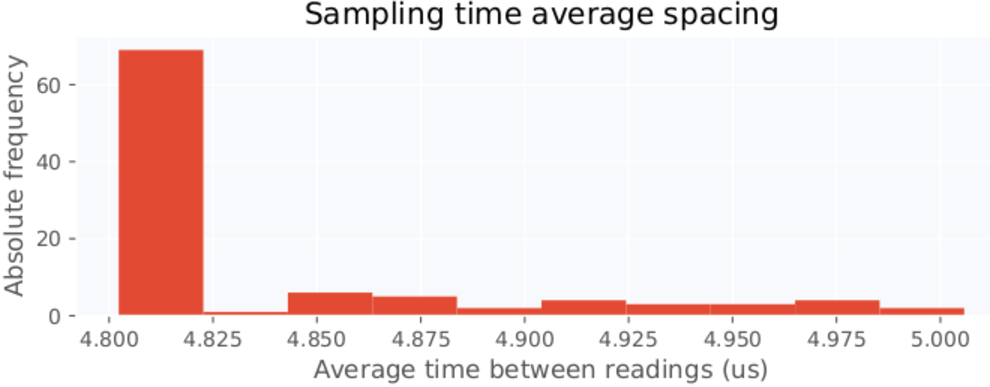
\includegraphics[width=0.65\textwidth]{samplingrate.pdf}
    \caption{$\Delta T / N$) in the real data-taking for $\sim 100$ signals. The average time difference is $(4.842 \pm 0.052) \mu s$, which corresponds to a rate of $(206.5 \pm 2.2) kHz$}
\end{figure}
\subsubsection{DAQ procedure}
Every acquired sample is put in a circular buffer of 3333 elements, which corresponds to a recording time of 16 ms. After the trigger, 2667 samples are acquired, until the whole buffer (which also contains 666 samples acquired before the trigger) is sent, as bytes, to the USB port connected to the PC.
The buffer was dimensioned (before the implementation of the trigger) to record 10 ms of data at the original sampling rate of 333 kHz.
\\
The time needed to transmit the data over the USB is the dead time of our DAQ procedure, and is of the order of 5 ms, as shown in figure.
\begin{figure}[H]
\centering
    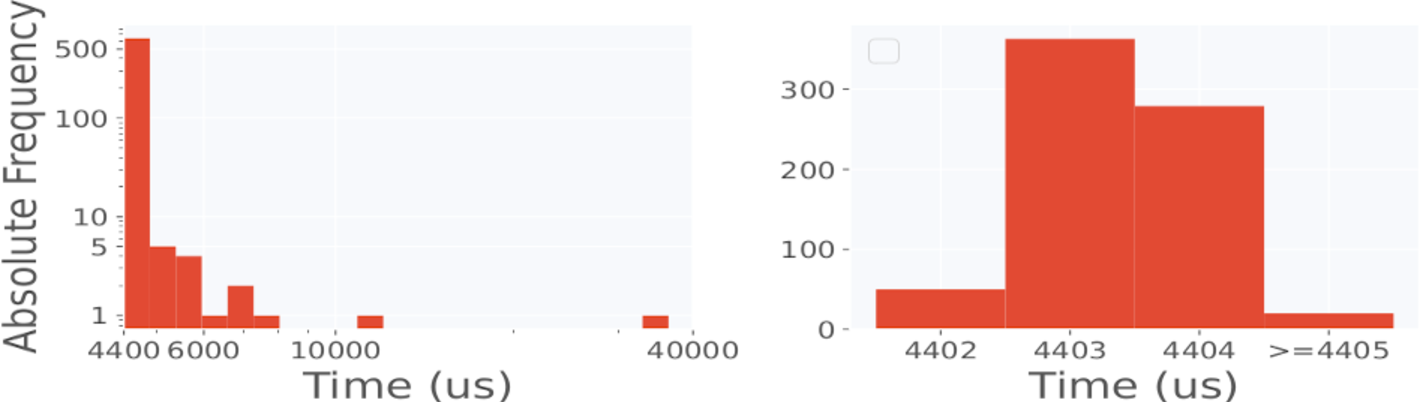
\includegraphics[width=0.9\textwidth]{dead_time_hist.pdf}
    \footnotesize{\caption{Acquisition dead time histograms in a typical use case: the first one (in log-log scale) shows all the distribution, that contains many outliers due to OS disturbances, while the second shows only its major part}}
\end{figure}
The Python script, running on a laptop, decodes the data and saves them in a text files with three columns: I, Q (in ADC units, from 0 to 4095) and the timestamp of each sample (in microseconds from the beginning of the data taking).\\
It is important that the script and the Arduino program are somehow synced. This is achieved through an handshake procedure, in which the script sends to Arduino the acquisition time duration, and receives back the trigger threshold. In this way not only these two useful piece of information are shared, but also Arduino starts sending bytes only when the script is ready to receive them, in order to avoid dangerous misalignments.
\begin{figure}[H]
\centering
% Define block styles
\tikzstyle{decision} = [diamond, draw, fill=blue!20, 
    text width=7em, text badly centered, node distance=4cm, inner sep=0pt, aspect = 2]
\tikzstyle{block} = [rectangle, draw, fill=blue!20, 
    text width=8em, text centered, rounded corners, minimum height=4em]
\tikzstyle{line} = [draw, -latex']
\begin{tikzpicture}[node distance=3cm, auto]
    % Place nodes
    \node [block] (init) {Handshake};
    \node [block, right of=init, node distance=5cm] (one) {Acquire one sample and save it in the buffer};
    \node [decision, right of=one, node distance=6cm] (trigger) {Trigger?};
    \node [block, below of=trigger] (many) {Acquire and save in the buffer (loop)};
    \node [block, below of=one] (write) {Write to USB all the buffer};
    % Draw edges
    \path [line] (init) -- (one);
    \path [line] (many) -- (write);
    \path [line] (write) -- (one);
    \path [line] (one) -- (trigger);
    \path [line] (trigger.north) |- node [near start] {no} ++(0,0.5cm) -|  (one);
    \path [line] (trigger) -- node {yes}(many);
\end{tikzpicture}
\caption{DAQ flow chart}
\end{figure}
Another important and annoying point is that the laptop must be disconnected from the power supply, so as to avoid the noise from the 220V line (caused by unresolved grounding issues), which affects the Arduino ADC reference voltage and makes the recorded data useless, as we have experienced during the first tries. 
\section{Data Analysis}
\subsection{IQ mixer calibration}
To calibrate the IQ mixer in the real experimental situation, we connected the apparatus to the KID and operated a frequency sweep in the range 2.555-2.558 GHz, which contains the resonance frequency 2.556326 GHz. The resulting ellipse in the I-Q plane was fitted, getting the parameters:
\begin{itemize}
\item I and Q offset: $I_c = 1.5742 V$ and $Q_c = 0.6235 V$
\item I and Q axis: $I_a = 0.4110 V$  and $Q_a = 0.4306 V$
with a resolution of 1 part over 1000.
\end{itemize}
\begin{figure}[H]
\centering
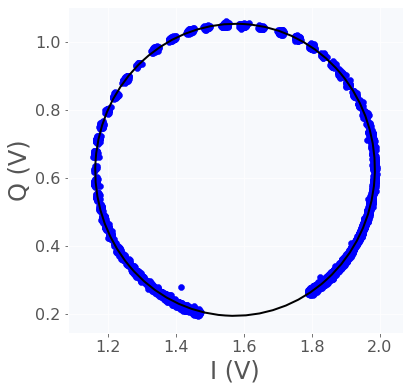
\includegraphics[width=0.5\textwidth]{ellipse.png}
\caption{Ellipse fit in the I-Q plane.}
\end{figure}
After subtracting the I and Q offset, the I-Q unbalance of the IQ mixer is corrected scaling the Q values by the ratio of the I and Q axis, by means of the formulas:
\begin{align}
& Q \to \frac{I_a}{Q_a}(Q-Q_c) \\
& I \to I - I_c
\end{align}
This converts our ellipse into a circle, therefore the phase can be evaluated simply as:
\begin{equation}
\phi = \arctan \left( \frac{Q}{I} \right)
\end{equation}

\subsection{Signals reconstruction}
The detector response in energy is proportional (in a certain range) to its response in phase and amplitude. We chose to analyze the events using only the heights of the phases pulses with respect to the baseline, estimated as the average over the first 500 points of each acquisition, which most probably do not contain pulses because the post-trigger samples are located after the 667th sample of each acquisition.
\subsubsection{Signal sources}
We analyzed the detector response to three types of energy deposition:
\begin{itemize}
\item Unavoidable cosmic rays passing through the absorber and natural radioactivity, not analyzed in detail.
\item X-rays coming from a very low-activity Fe-55 source on the absorber. This isotope decays via electron capture to Mn-55 with a half-life of 2.737 years. It emits Auger electrons of 5.19 keV, with a probability of about 60\%, K-alpha-1 X-rays of 5.89875 keV with a probability about 16.2\%, K-alpha-2 X-rays of 5.88765 keV with a probability of about 8.2\%, or K-beta X-rays of 6.49045 keV with a probability of about 2.85\%. The energies of the K-alpha-1 and -2 X-rays are so similar that they are often specified as mono-energetic radiation with 5.9 keV photon energy and probability of about 28\%. The remaining 12\% is accounted for by lower-energy Auger electrons and photons from minor transitions. Unfortunately our apparatus is not capable of distinguishing the peaks, because all of them are very spread (more than our detection resolution), due to the geometry of the source and detector. Moreover, the Auger electrons are not detectable because a plastic film (scotch) covers our source.
\item 400nm light pulses, sent to the resonator in 50ms-spaced bunches via an optical fiber. The light source is controlled through a signal generator in burst mode, so that the number of photons $n$ in each bunch, which represents the light intensity, is proportional to the easy to set number of pulses in the bursts.
\end{itemize}
\begin{figure}[H] 
        \centering 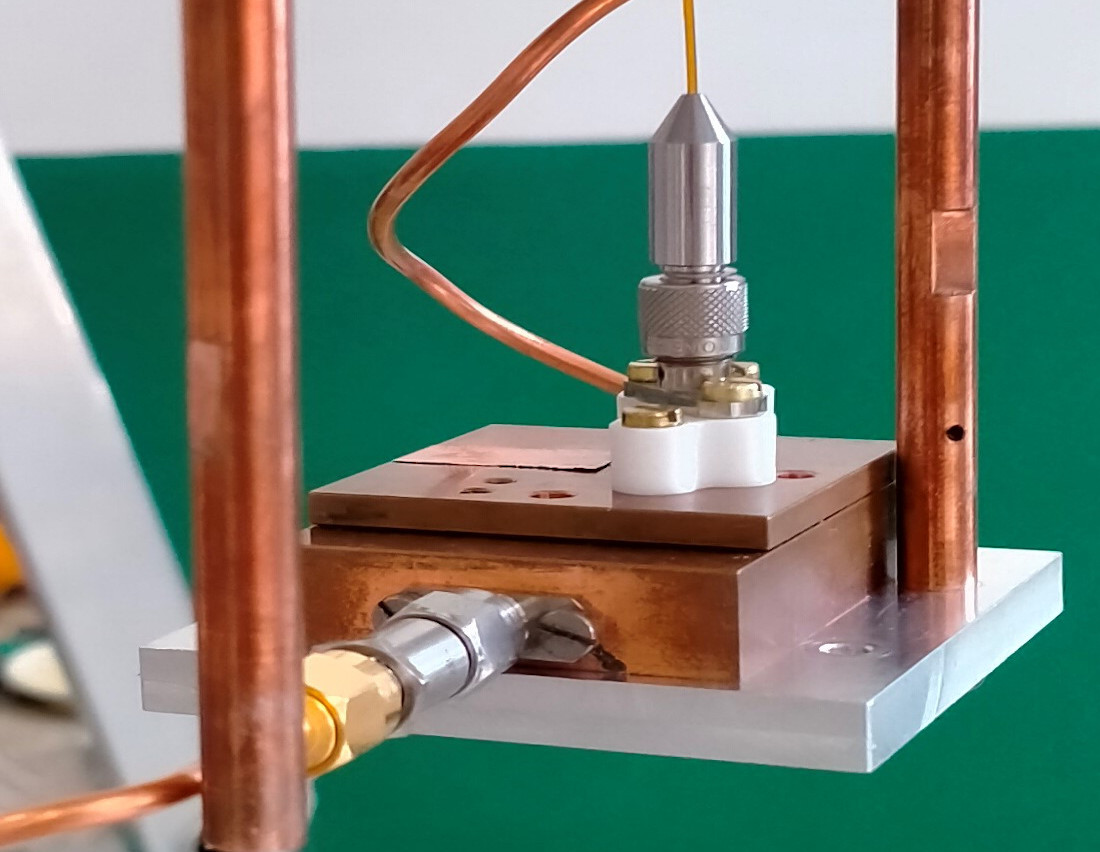
\includegraphics[width=0.5\textwidth]{kid_fibra.jpg}
        \caption{
               KID apparatus, with the optical fiber and the radioactive source on top.
        }
\end{figure}
\subsubsection{Smoothing}
In order to carefully evaluate the phase pulses height, we firstly need to smooth the signals and to select in a better way the events. The way this should be done is determined by the noise spectral density, reported in figure:
\begin{figure}[H]
\centering
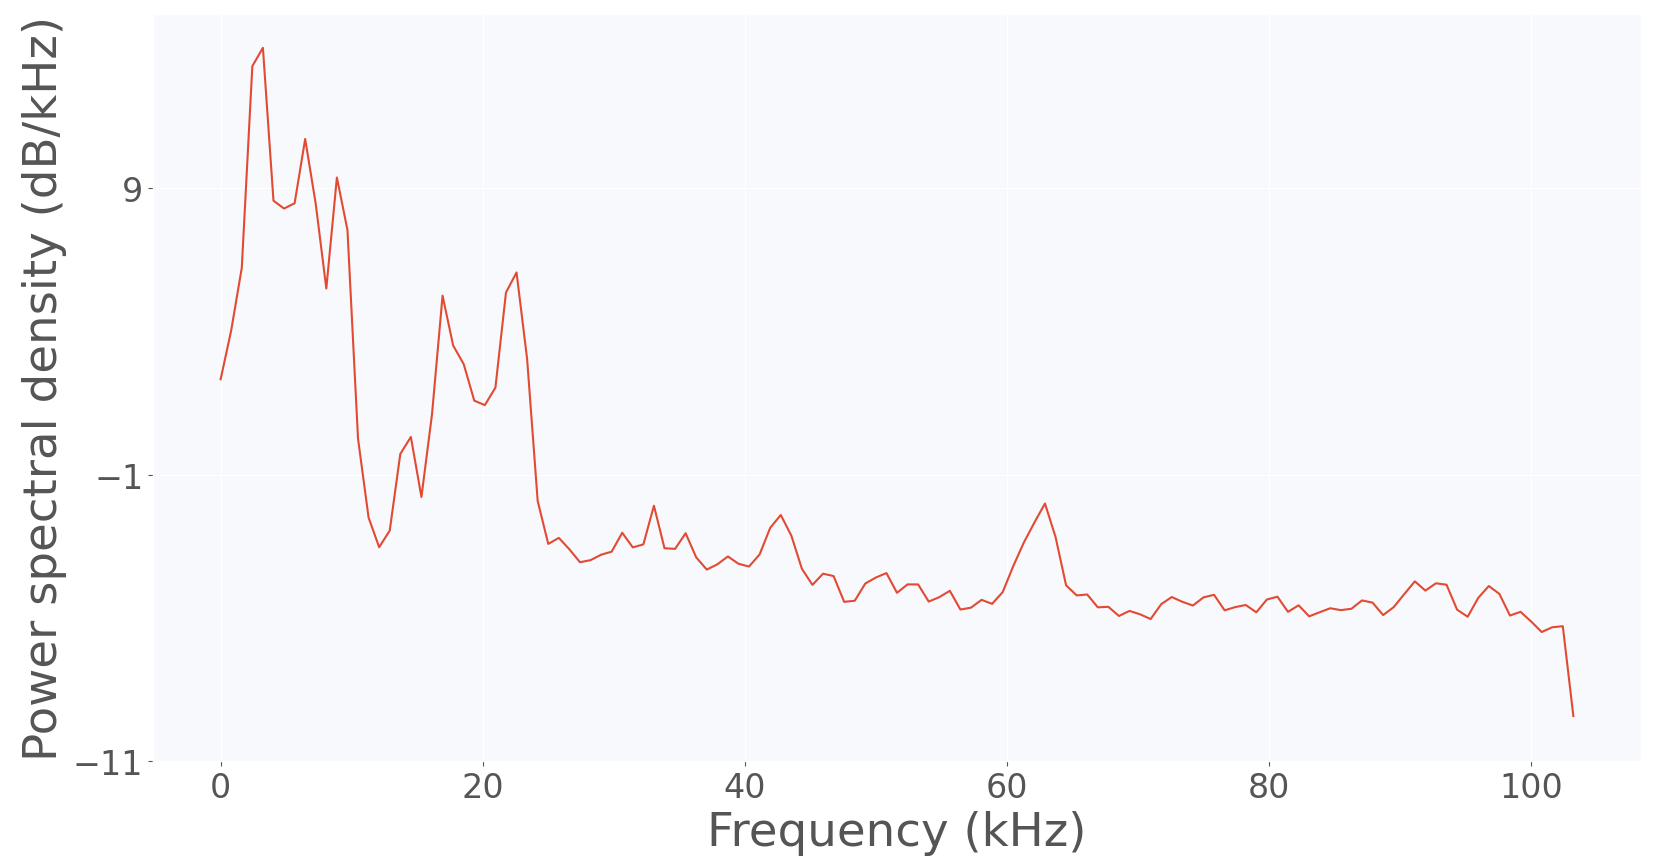
\includegraphics[width=0.7\textwidth]{spectral density.png}
\caption{Phase noise spectral density. Note that the noise has been retrieved by the pre-pulse window of 666 samples in each file.}
\end{figure}
The two most noisy region are located nearly 2.5 kHz and 20 kHz, which are in the same region of signal characteristic frequencies. We then need just to smooth the signals, in order to keep the pulses visible and to suppress the noise. For the sake of simplicity we chose to use a moving average with a window of 70 points, as shown in figure. 
\begin{figure}[H]
\centering
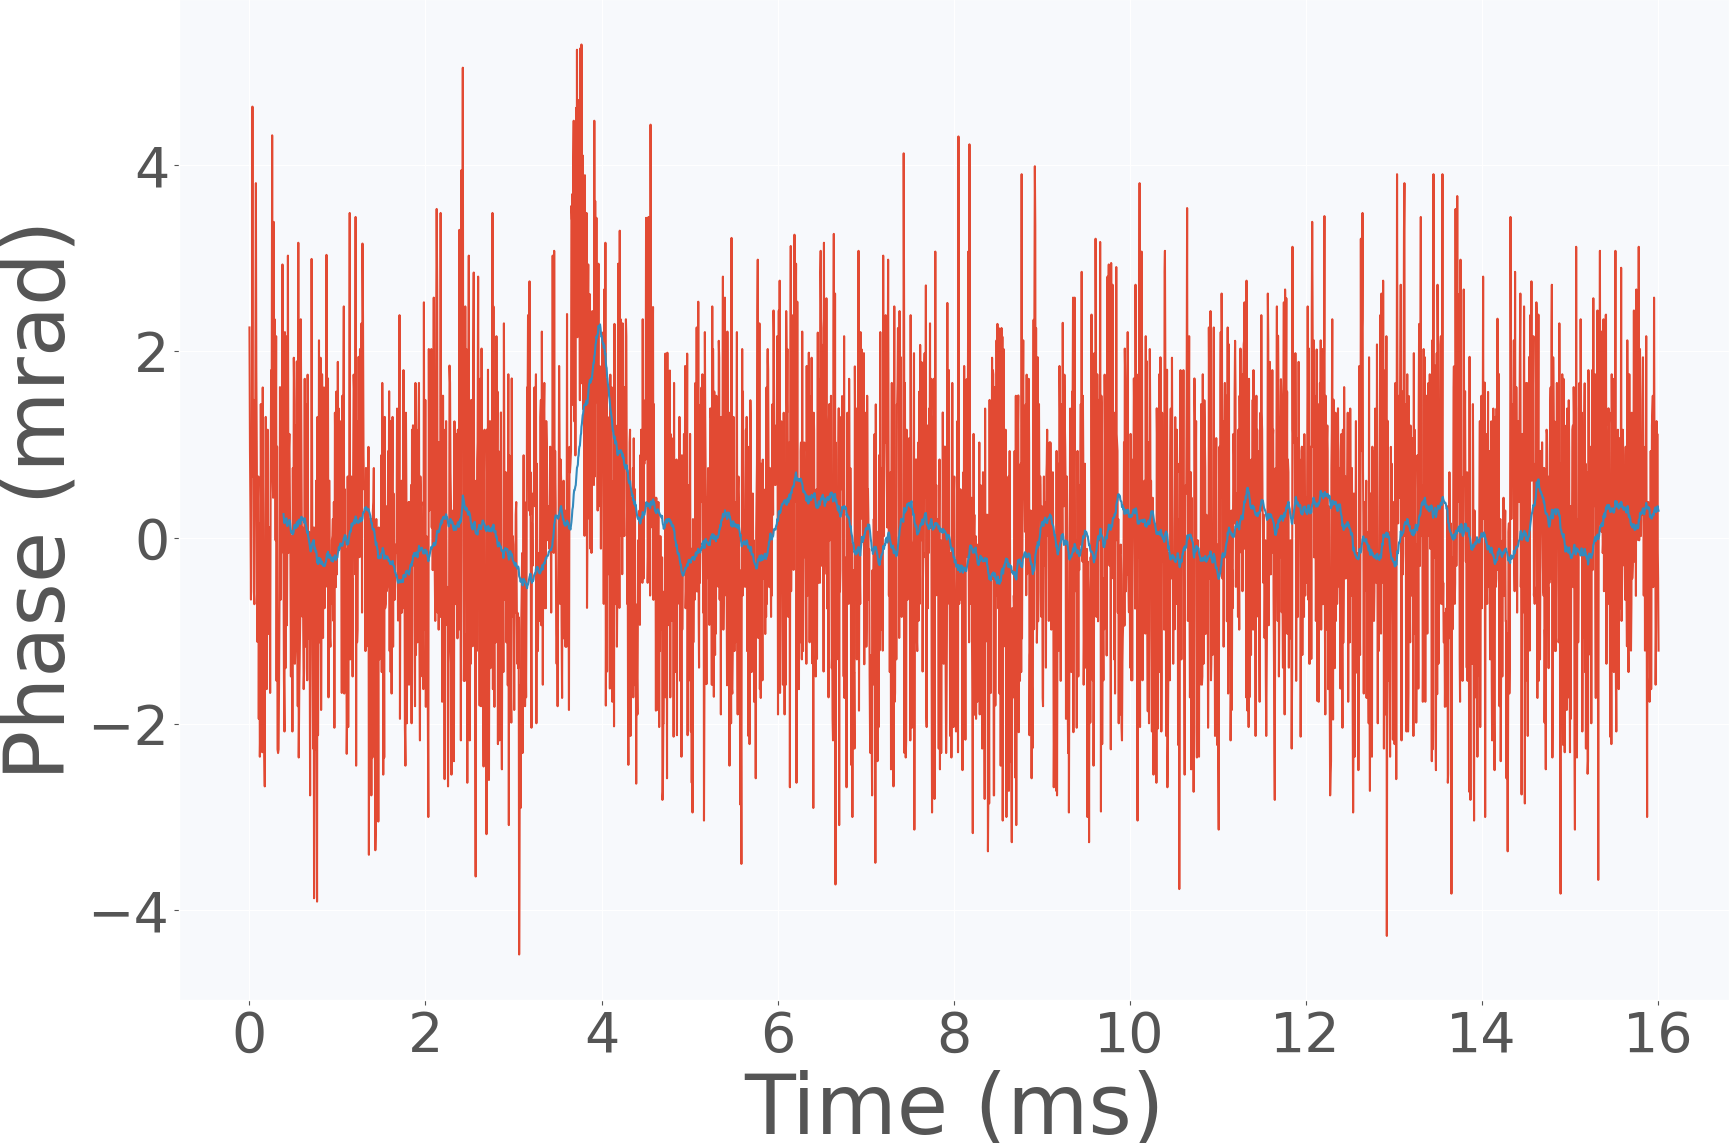
\includegraphics[width=0.32\textwidth]{figure1.png}
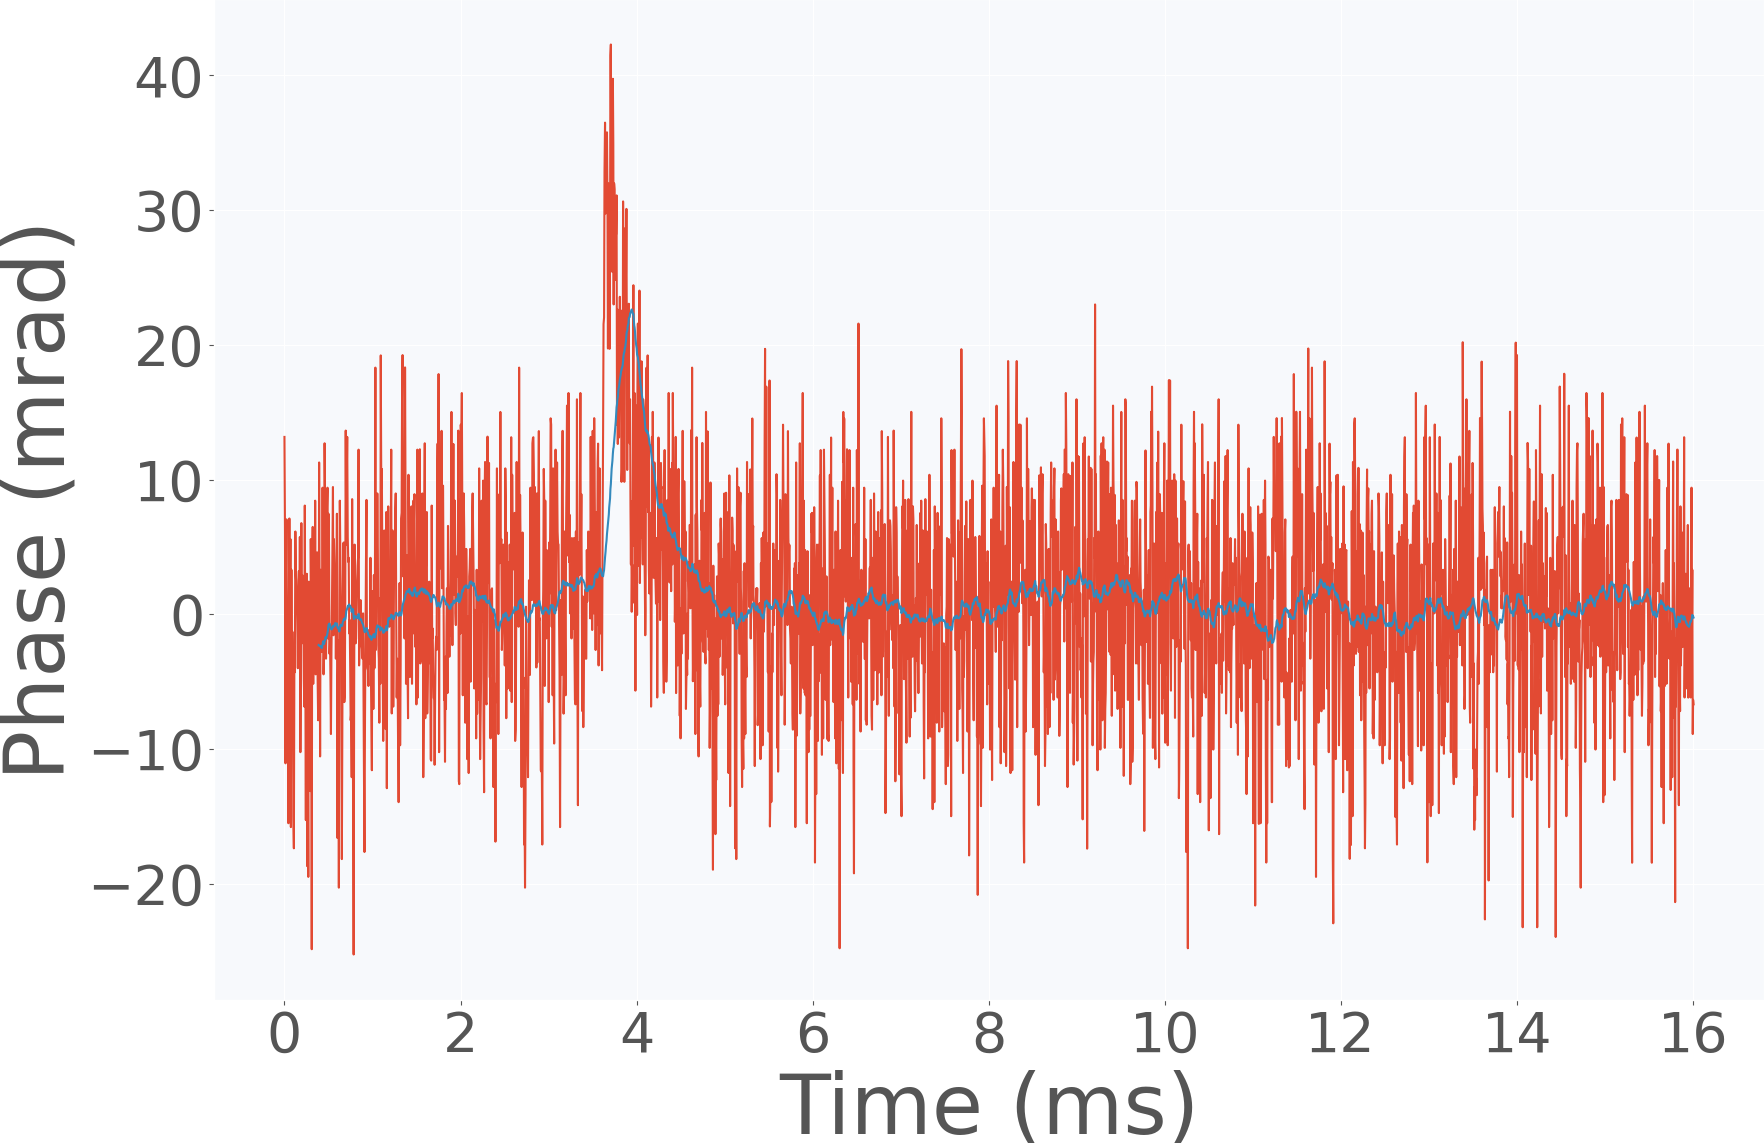
\includegraphics[width=0.32\textwidth]{figure2.png}
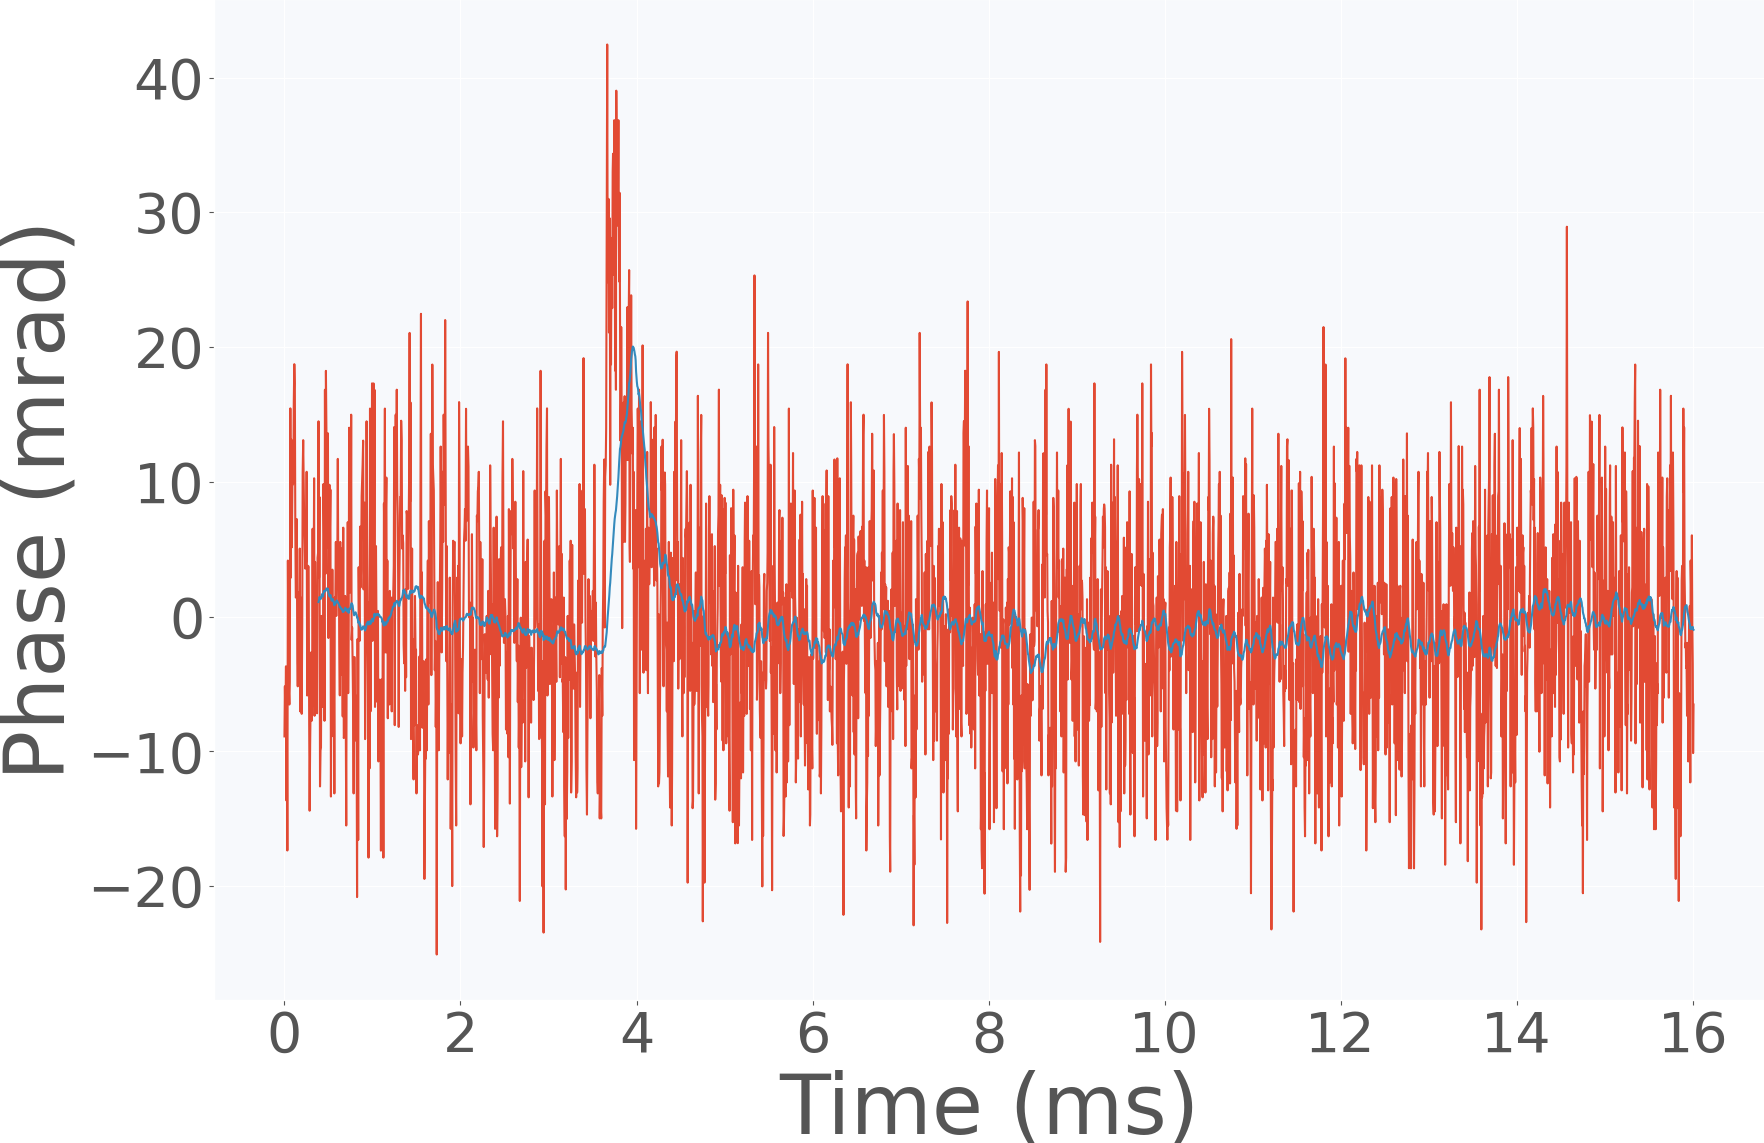
\includegraphics[width=0.32\textwidth]{figure3.png}
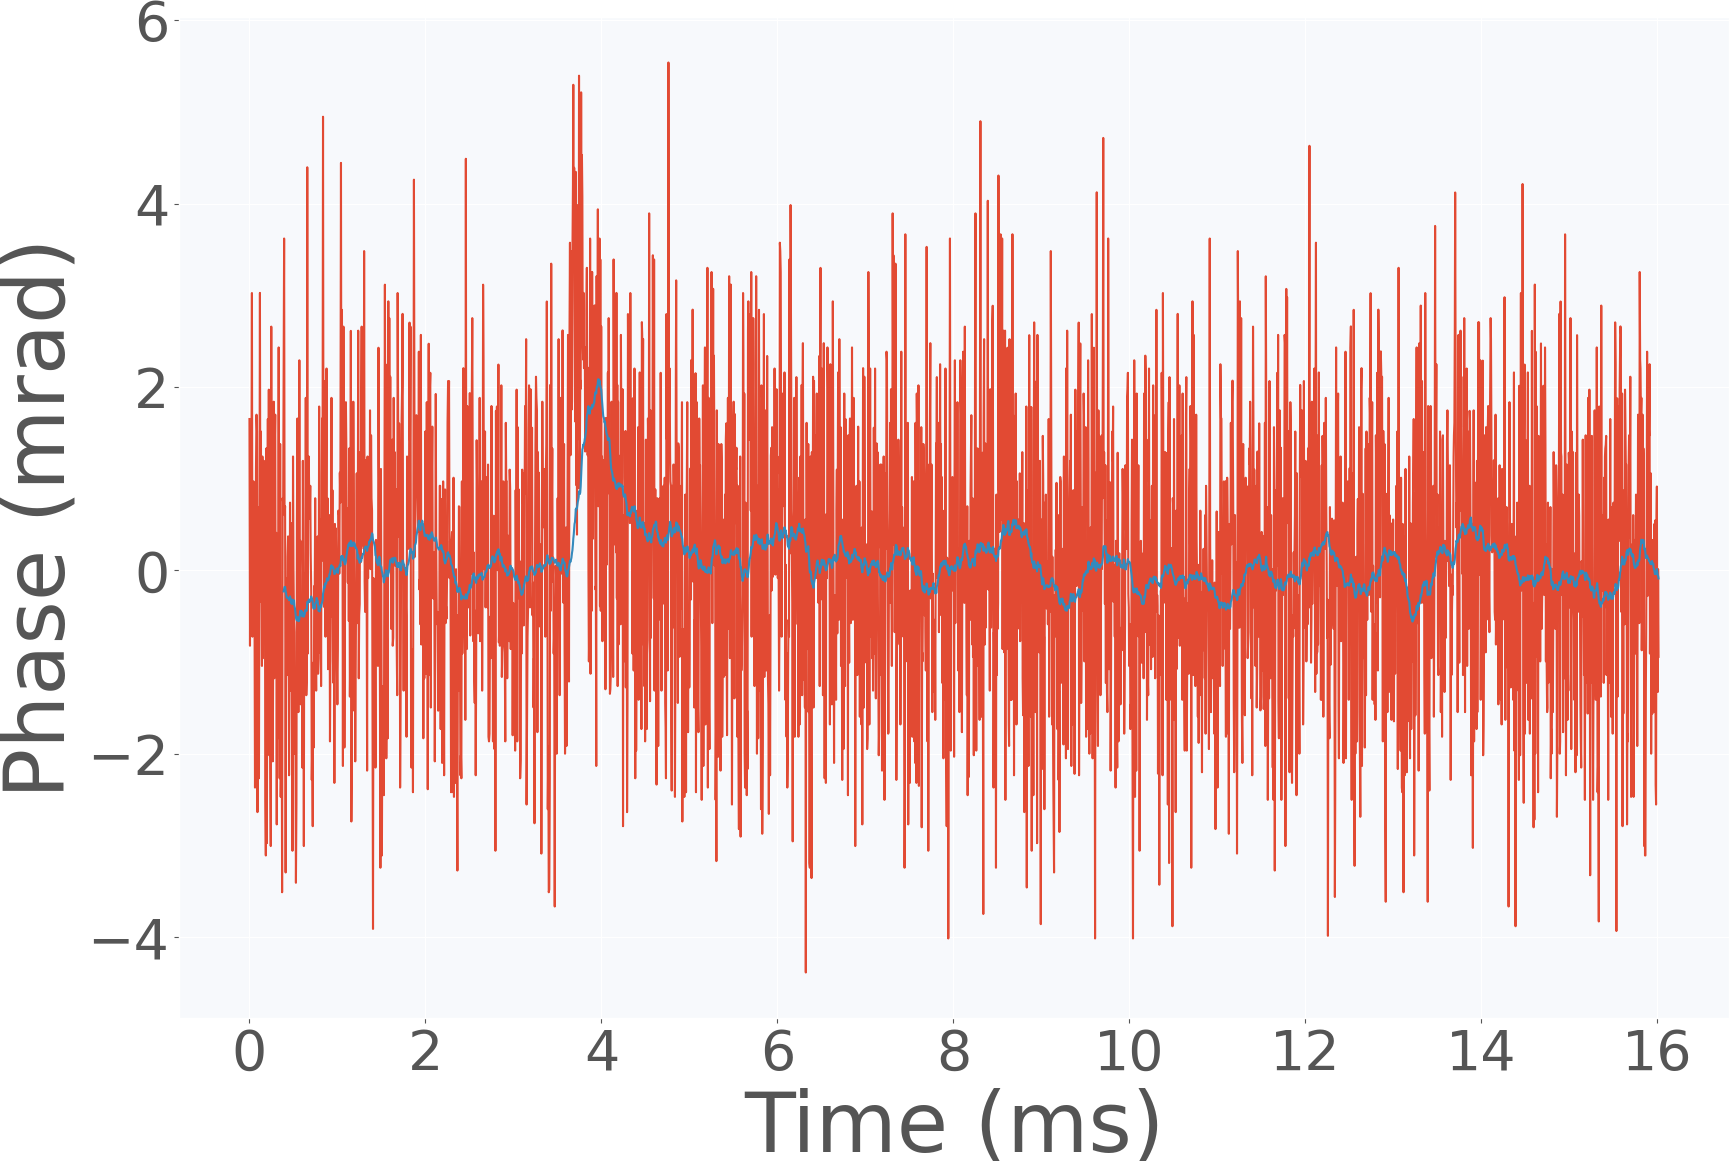
\includegraphics[width=0.32\textwidth]{figure4.png}
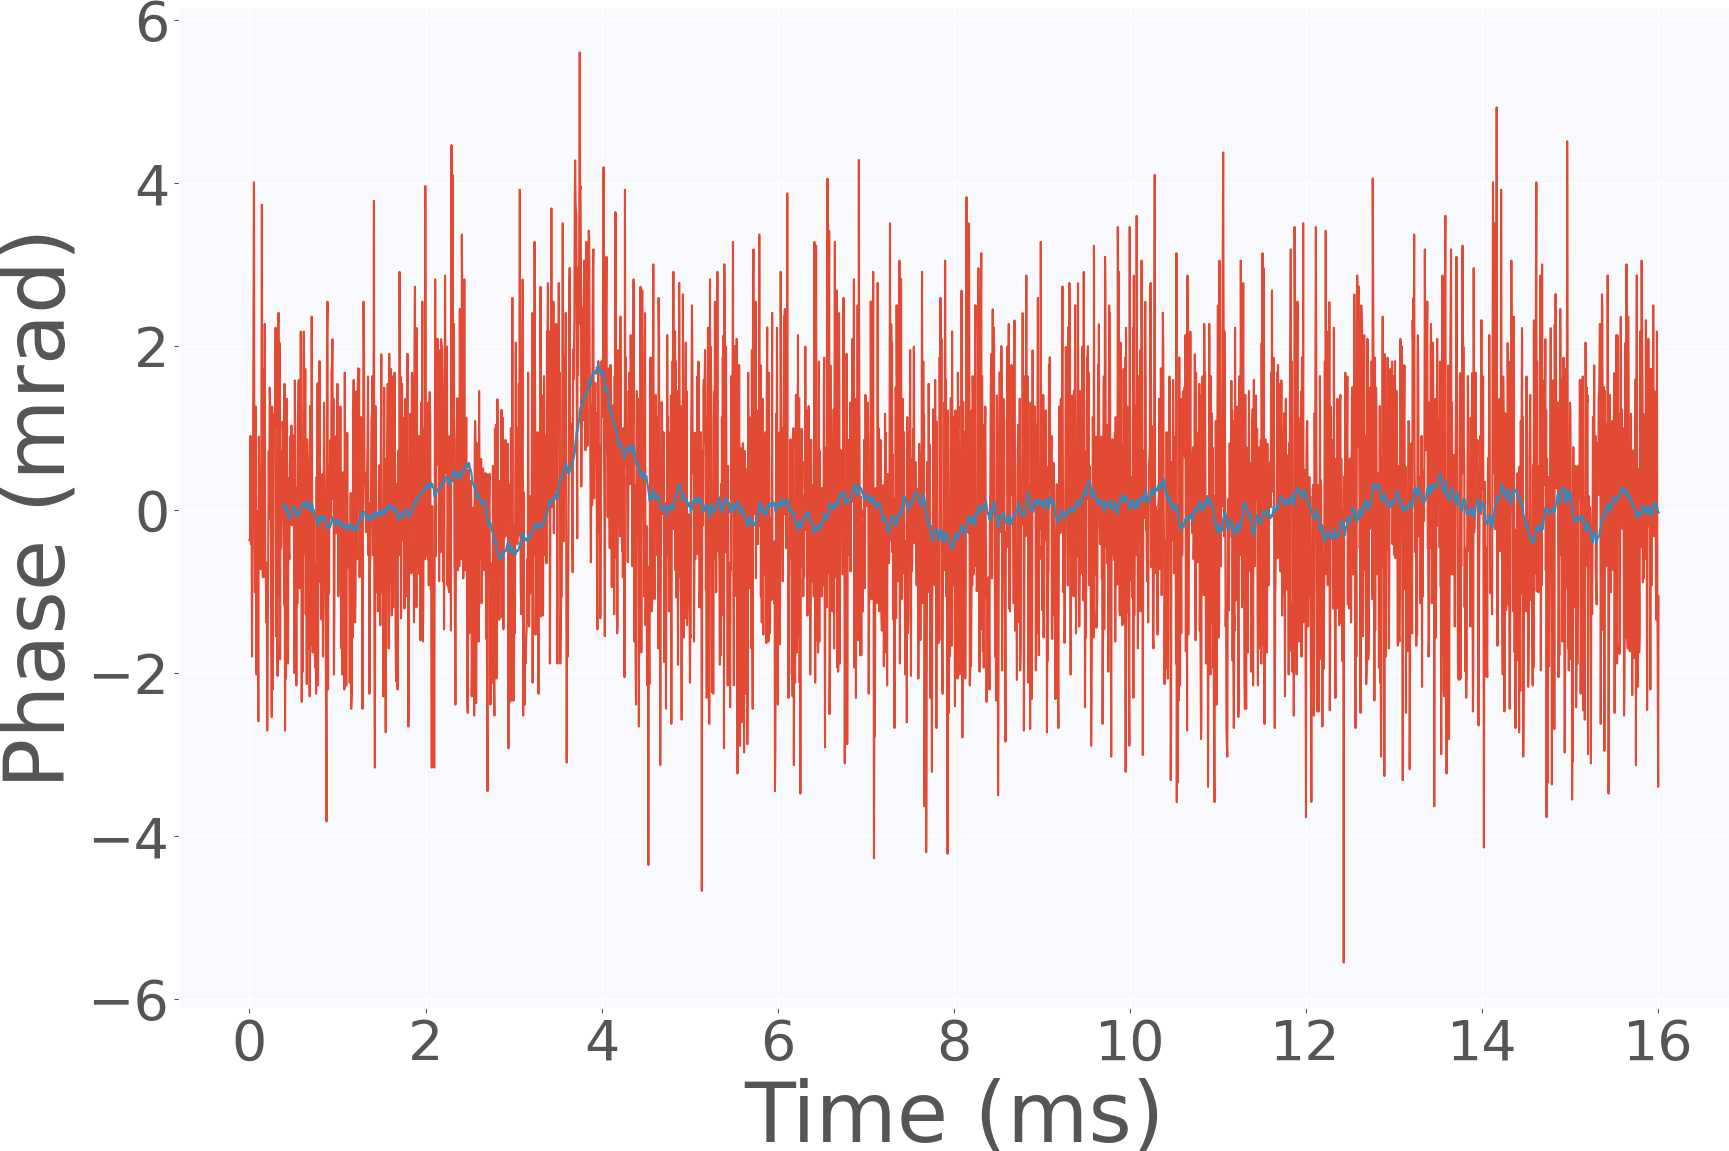
\includegraphics[width=0.32\textwidth]{figure5.png}
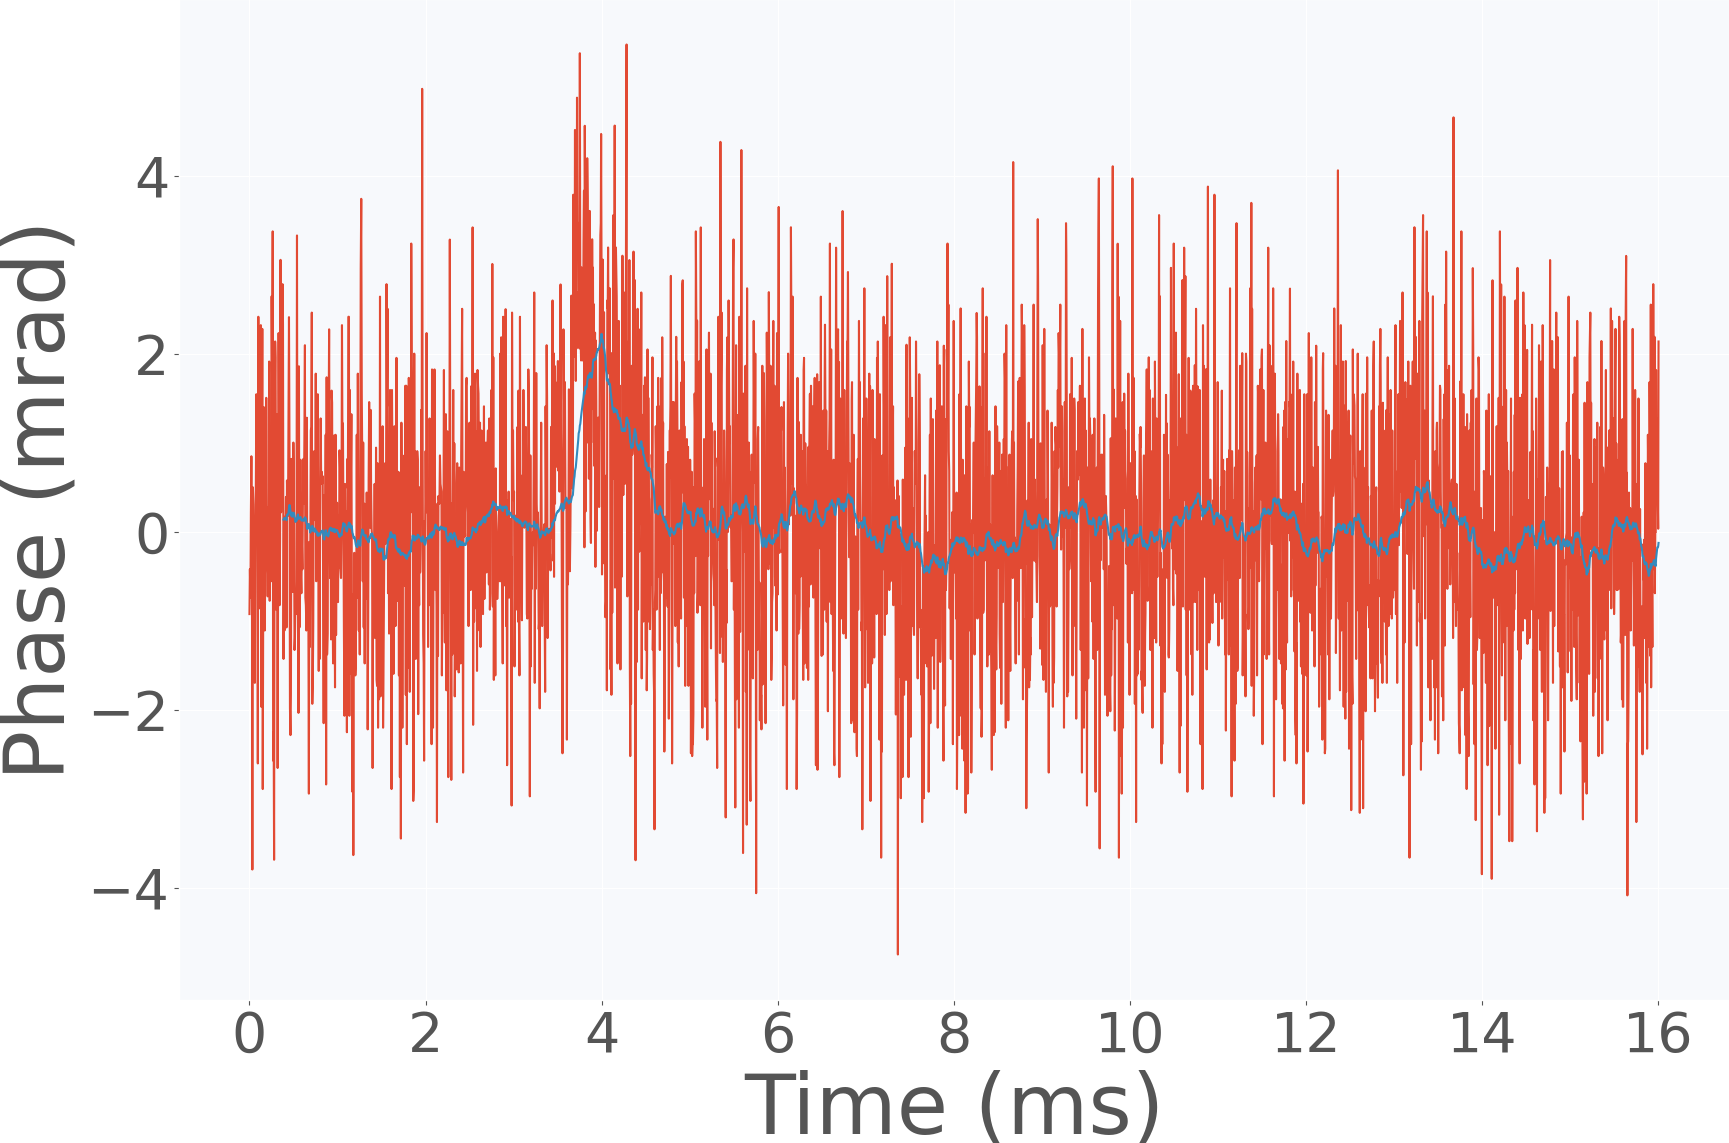
\includegraphics[width=0.32\textwidth]{figure6.png}
\caption{Some of the smallest pulses selected, showing in red the non-smoothed phase waveform and in blue the smoothed one.}
\end{figure}
The value of 70 for the window has been chosen because it provided a good uncertainty on the phase response to light pulses, as shown in figure.
\begin{figure}[H]
\centering
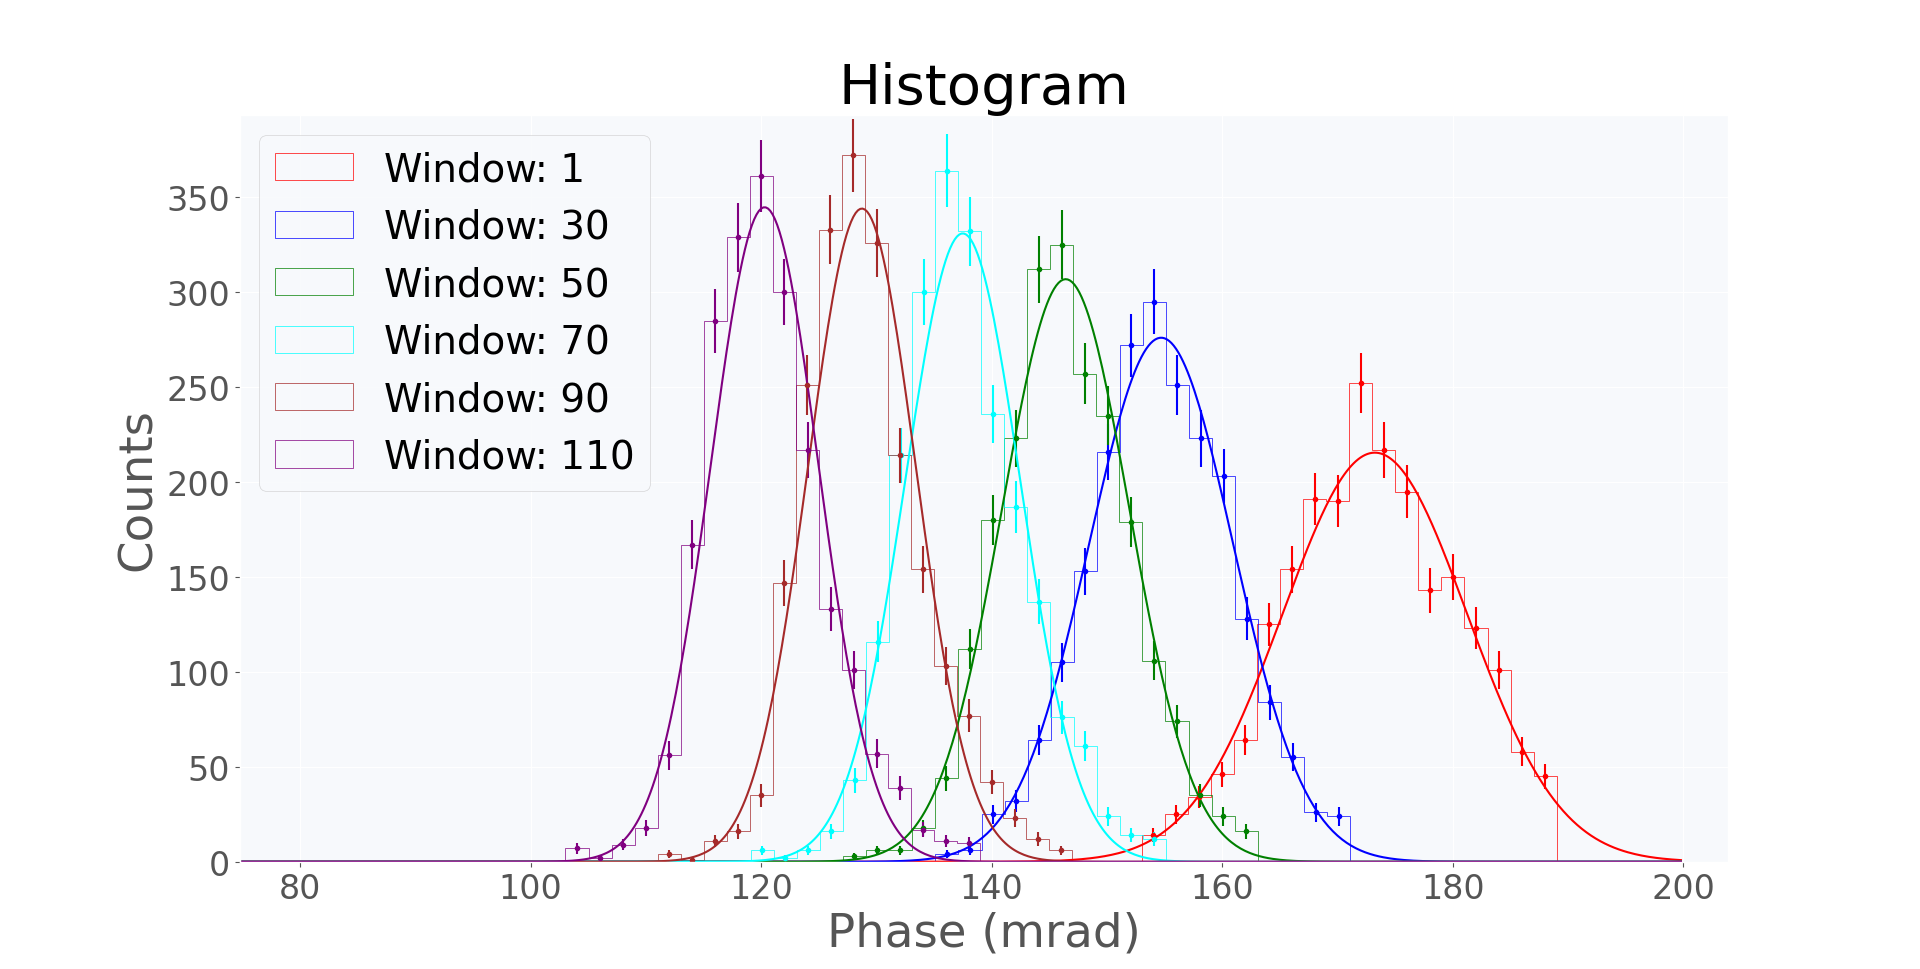
\includegraphics[width=0.9\textwidth]{choose_window.png}
\caption{Histograms of phase response to light pulses (2 cycles) for several different windows, fitted with gaussians. The uncertainties with a window of 70, 90 or 110 are extremely similar, so we decided to use a window of 70 in order to have a faster time response.}
\end{figure}
As the pulses height is lowered by this smoothing procedure, we must multiply them by a gain factor, which is the average ratio between the height of the non smoothed peak and the smoothed one. This factor is equal to $1.296 \pm 0.002$ for a window of 70.
\subsubsection{Events selection}
The Arduino online trigger is not sufficient for our purposes, as it only provides a rough but very permissive trigger able to reduce the amount of data to handle.\\
However, our real event selection is based on the same method, working with the phases instead of the I values.\\The window of the rolling mean and the step of the derivative, which are equal to 10 in the online trigger, are kept both equal to 70, so we only have one parameter to optimize: the threshold.\\
First of all we recorded data for about 30 minutes (at the middle of June) without sending light pulses and visually selected the real events (the ones with a visible pulse in the waveform) out of the first 1000 files (16 ms acquisitions) obtained.\\
Then we leveraged this visual selection to optimize the threshold using the precision-recall curve method. It consists of finding the thresholds that maximizes both the precision and the recall, defined as:
\begin{equation}
\text{Precision}={\frac {tp}{tp+fp}},\quad \text{Recall}={\frac {tp}{tp+fn}}
\end{equation}
where $tp$, $fp$ and $fn$ are, respectively, the true positive rate, the false positive rate and the false negative rate. In other words, in the recall-precision plane, we chose the threshold that minimizes the distance to the $(1, 1)$ point. As shown in figure \ref{fig: Prec}, the best threshold is $14$ mrad and it provides a precision of 99.7\% and a recall of 98\%.
\begin{figure}[H]
\centering
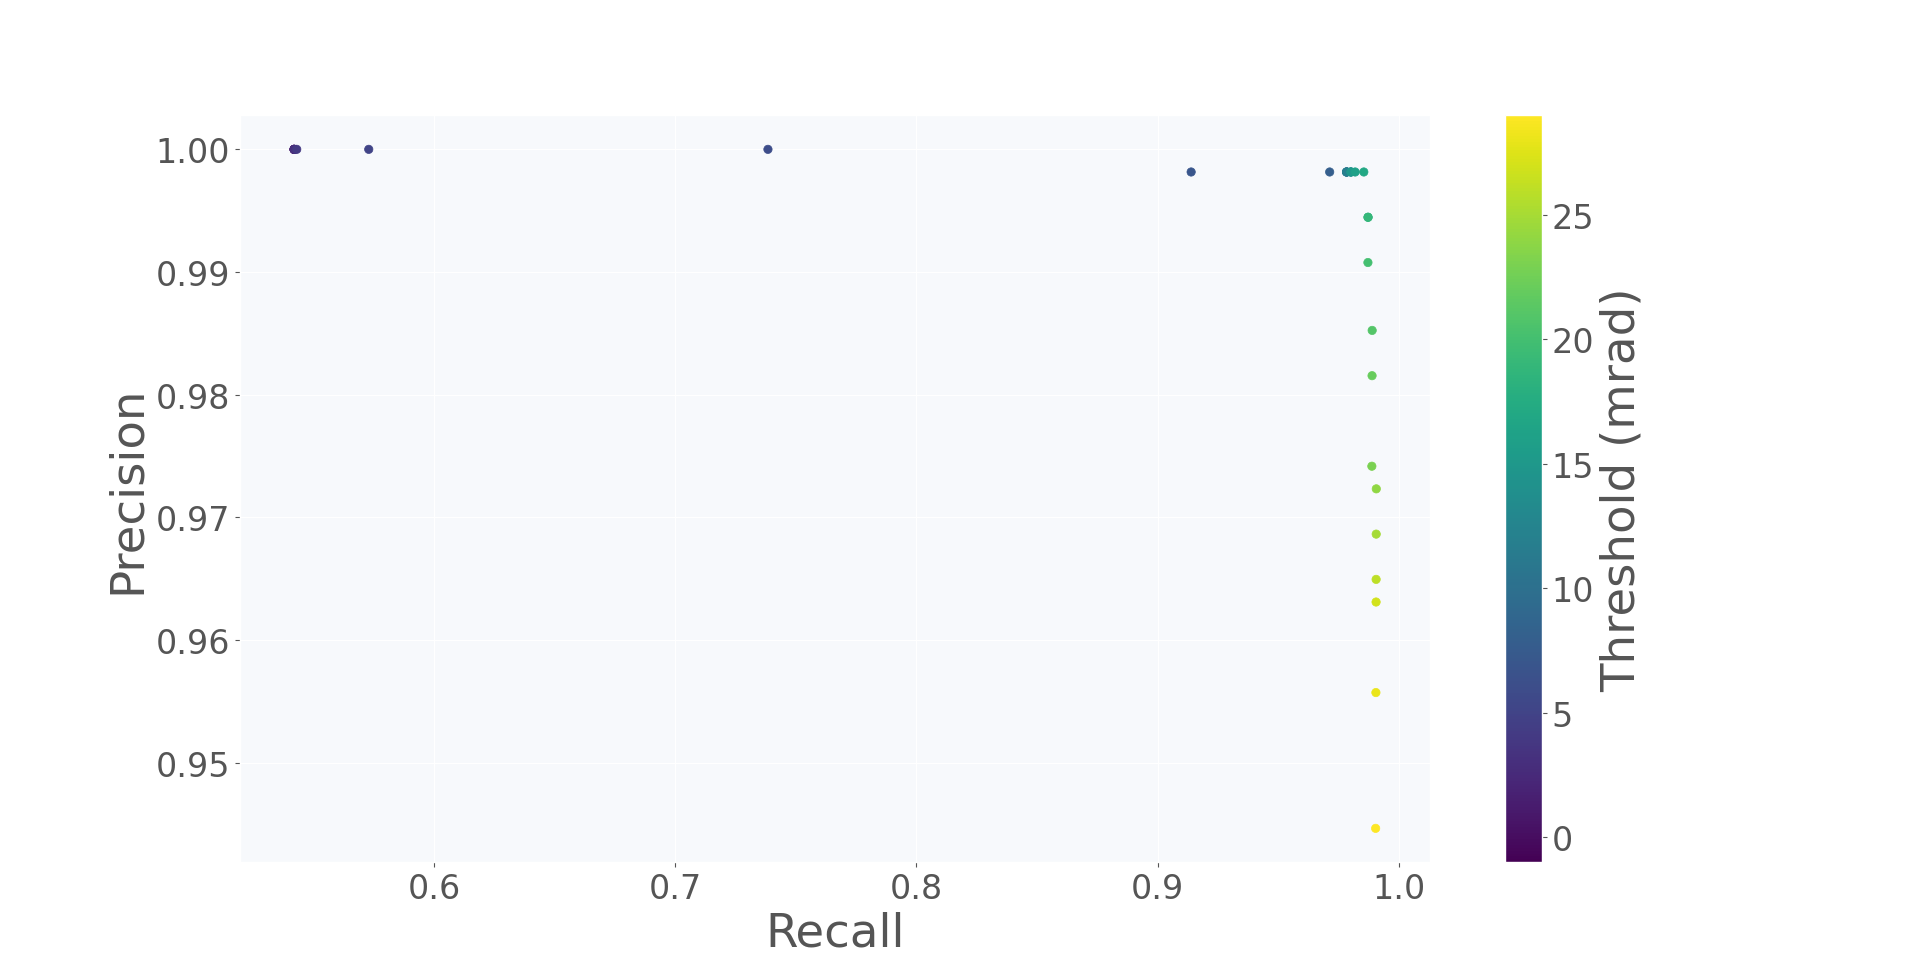
\includegraphics[width=0.9\textwidth]{prec-rec.png}
\caption{\label{fig: Prec}Precision-recall curve for 2000 acquisitions, with thresholds from 0 to 30.}
\end{figure}
\subsection{Calibration}
The phase response $\phi = \frac{d \phi}{dE} E$ is proportional to the incident energy $E$ in the detector, which is given by $\epsilon n$, being $\epsilon = 3.1 eV$ the photon energy at 400nm.\\
As $n$ (which is a huge number) is Poisson-distributed, $\delta E = \epsilon \sqrt{n}$, in the absence of other sources of error; then $\delta \phi = \frac{d \phi}{dE} \epsilon \sqrt{n}$. Writing $\phi$ as $\phi = \frac{d \phi}{dE} \epsilon n$, we can show that $\sigma^2[\phi] = \frac{d \phi}{dE} \epsilon \phi$. Including the effect of the finite resolution $R_\phi$ of the detector, we obtain:
\begin{equation}
    \sigma^2[\phi] = R_\phi^2 + \frac{d \phi}{dE} \epsilon \phi
\end{equation}
Thus, to calibrate our detector, we only need to send to the KID light pulses with different numbers of cycles, evaluate the expected value and the variance of the phase peaks for each one, and fit $R_\phi$ and $\frac{d \phi}{dE}$through the above formula.
The number of cycles sent was in the range $1-6$; unfortunately, due to DAQ problems, we had to discard the data-takings with 4 and 5 cycles. The mean and variance of the peaks has been estimated by fitting the histograms with gaussians, as shown in figure.
\begin{figure}[H]
\centering
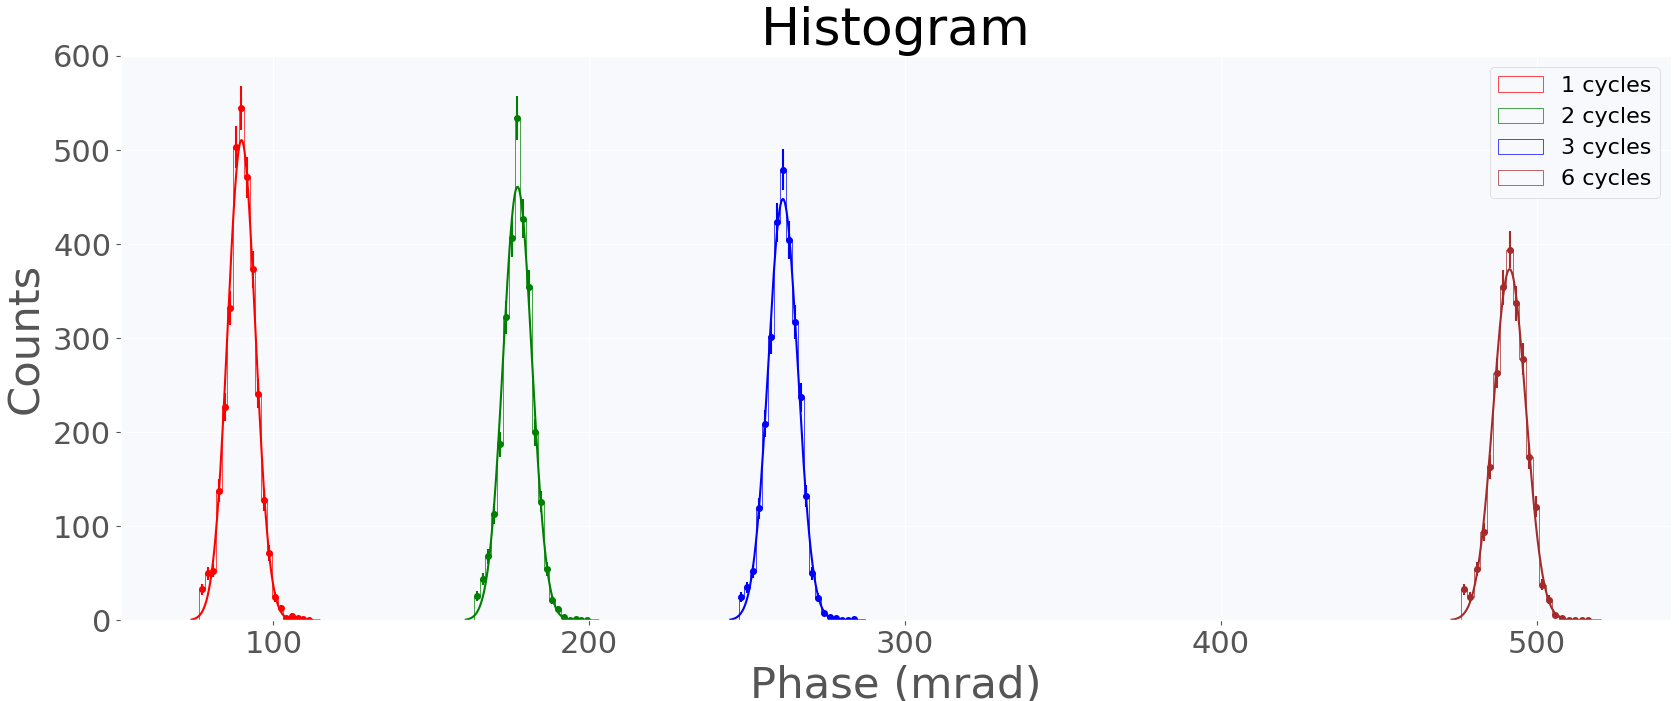
\includegraphics[width=0.7\textwidth]{hist_lungo.png}
\caption{Histograms of the phase response to the light pulses, with gaussian fit.}
\end{figure}
Before making the calibration linear fit, we verified the linearity of the response, as shown in figure. 

\begin{figure}[H]
\centering
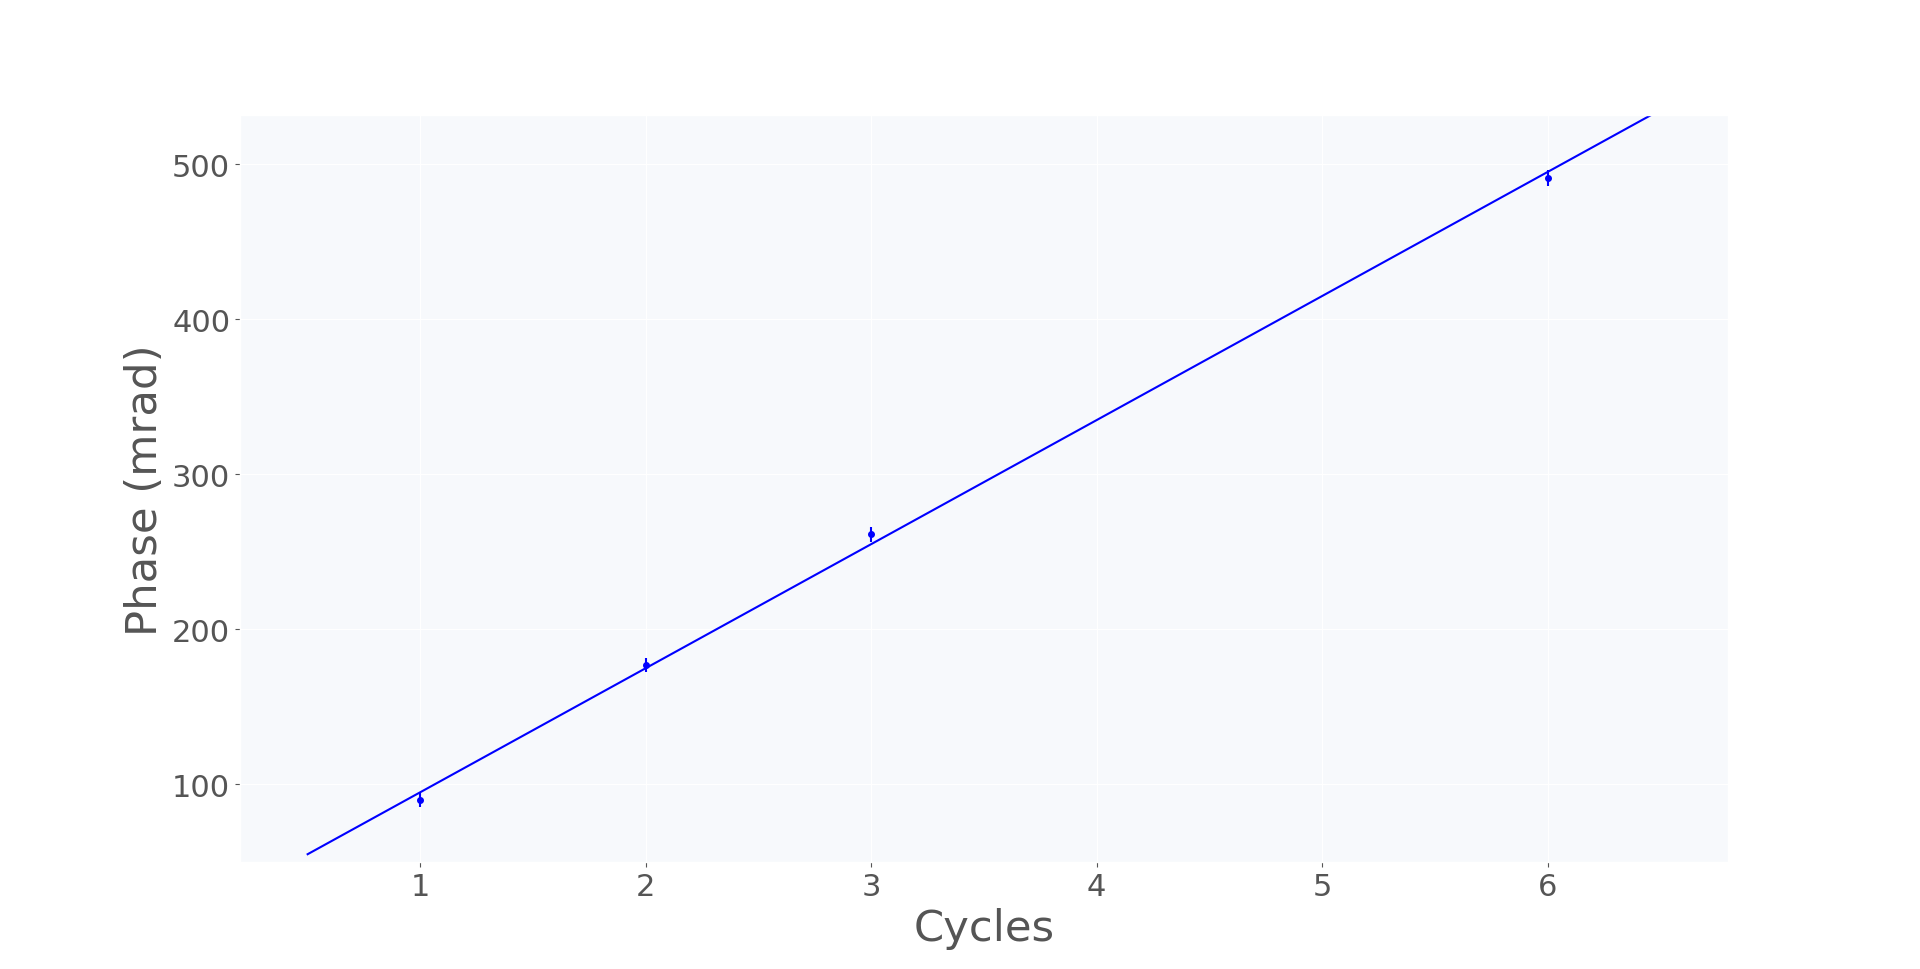
\includegraphics[width=0.8\textwidth]{calib_cycles_vs_phase.png}
\caption{Peaks mean vs. number of cycles, to verify the linearity of the response.}
\end{figure}
\begin{figure}[H]
\centering
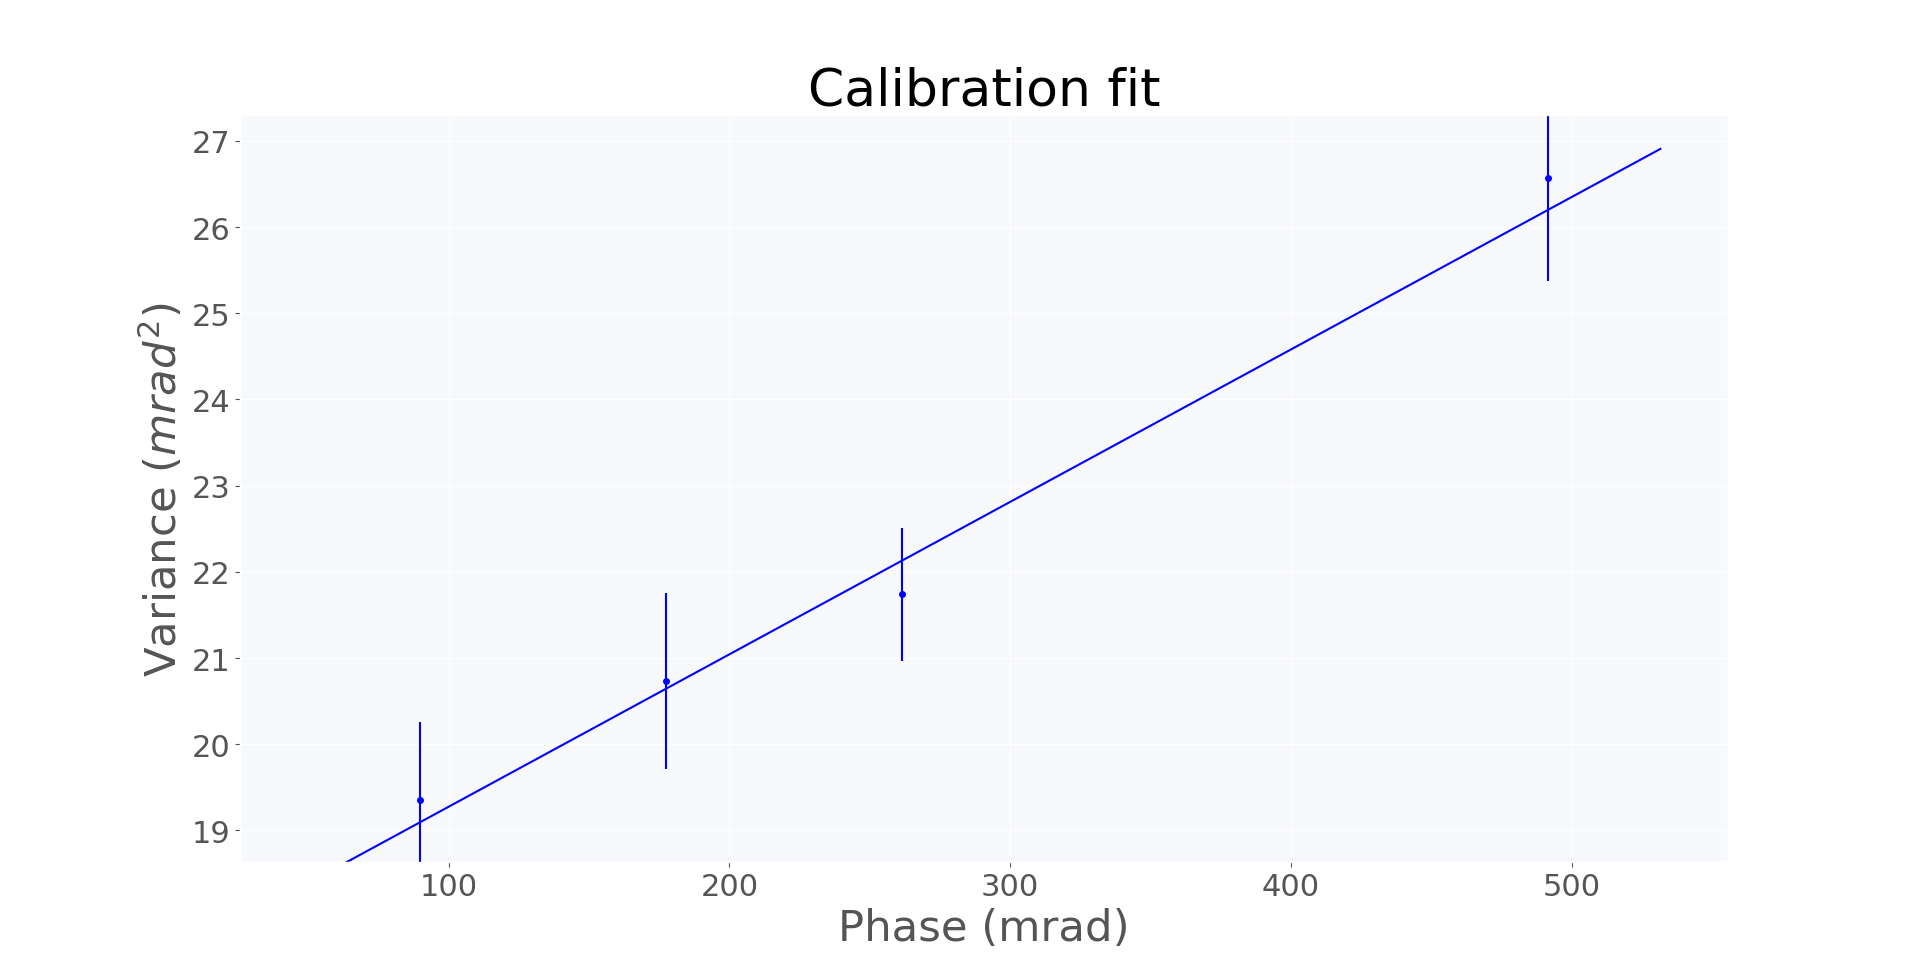
\includegraphics[width=0.8\textwidth]{calib_fit.png}
\caption{Calibration fit of $\sigma^2[\phi]$ vs. $\phi$.}
\end{figure}
We obtained a $\frac{d \phi}{dE}$ of $( 5.70 \pm 0.55)$ mrad/keV and a resolution in phase of $R_\phi = (4.183 \pm 0.054)$ mrad, corresponding to a resolution in energy of $(733 \pm 68)$ eV, which is very large compared to the result obtained in \cite{Cardani} (82 eV) using high-quality electronics.
\subsection{Fe-55 X-ray peak}
In a 30 minutes long data-taking we selected 1179 events, corresponding to a rate of 0.655 Hz. The histogram of the energy of these events reveals a peak at $(6.0 \pm 1.9)$ keV. The fact that this peak does not contain noise is verified by plotting another histogram of the same data-taking, where the events are selected with a more permissive threshold of $7$ mrad (instead of 14 mrad). The pedestal, as shown in figure, is only present with the lower threshold, is centered at about $0.8$ keV and does not overlap with the peak. The hypothesis that this peak corresponds to the K-alpha X-ray of Fe-55 (with a small unresolved component of K-beta X-rays) is consistent because its energy should be $5.89$ keV, which is perfectly compatible with the value fitted.
\begin{figure}[H]
\centering
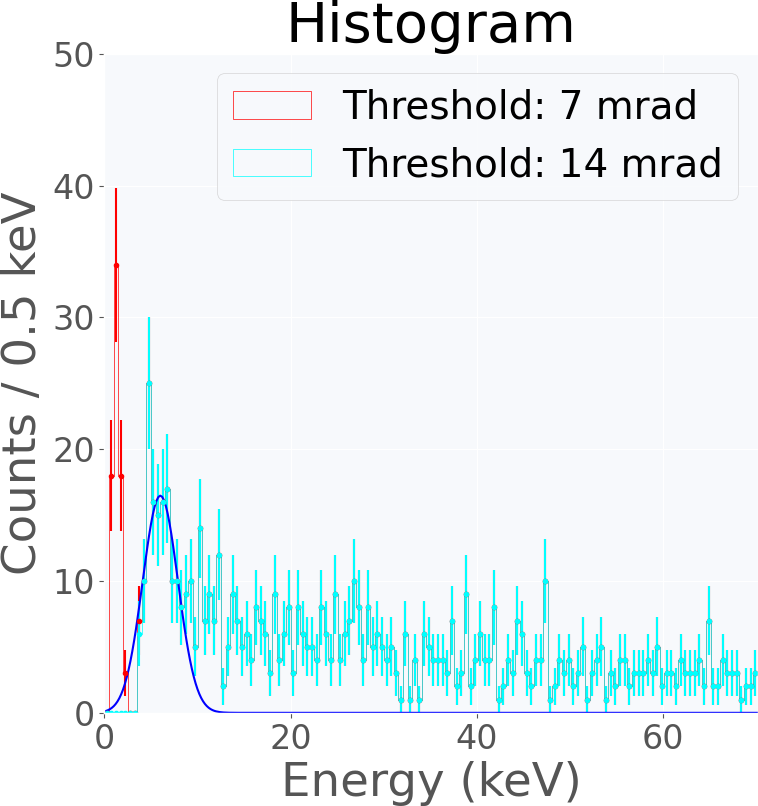
\includegraphics[width=0.49\textwidth]{Figure_1.png}
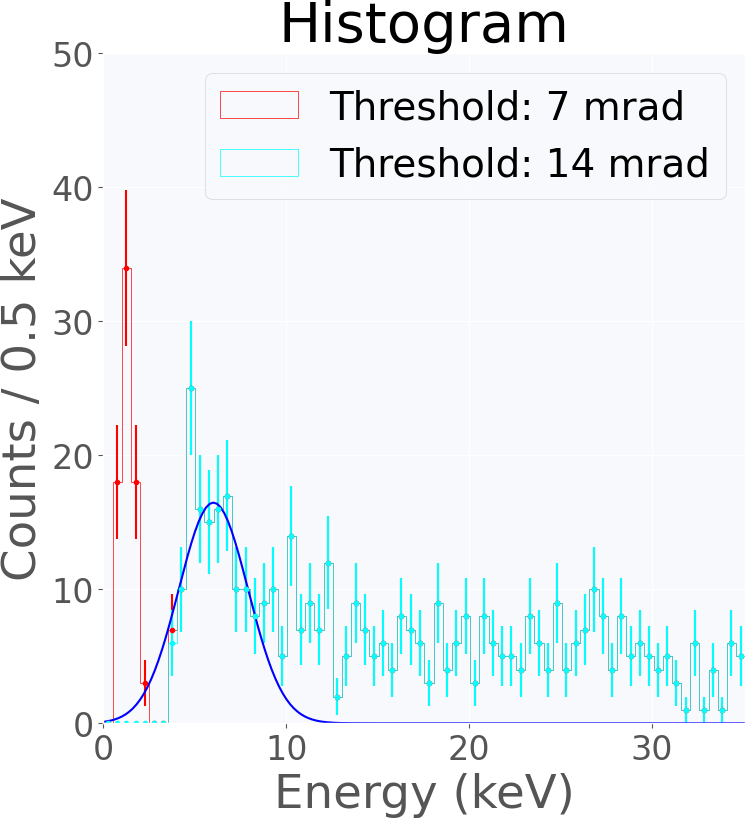
\includegraphics[width=0.48\textwidth]{Figure_2.png}
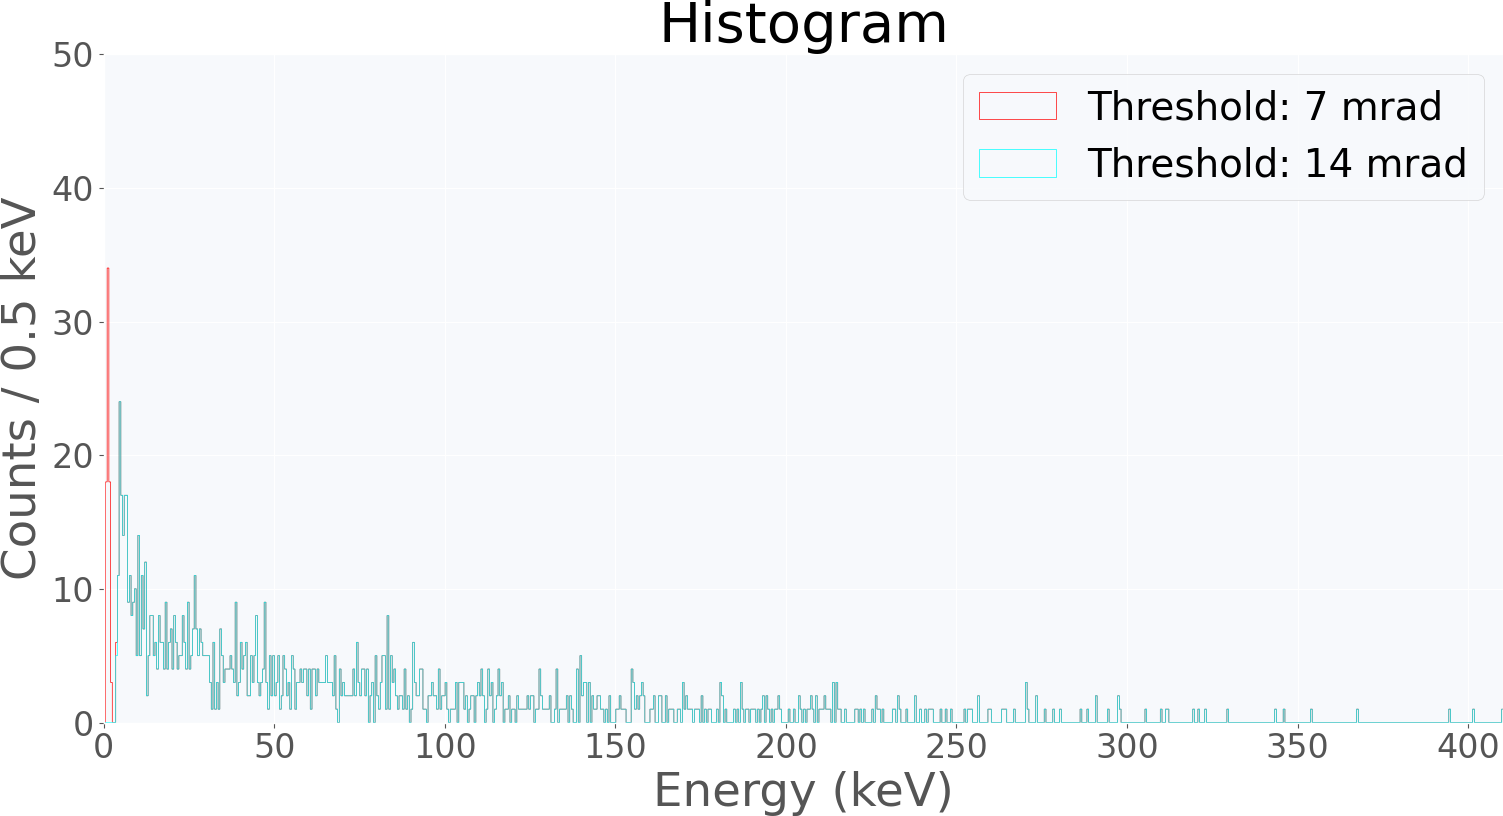
\includegraphics[width=\textwidth]{Figure_3.png}
\caption{Histograms of the selected events for different range of values. The last histogram was not plotted with uncertainties (given by the Poissonian distribution) for the sake of visual clarity. Note that after the pedestal the red and blue histograms overlap completely.}
\end{figure}
\section{Statistical Methods}
All the fit without errors on the indipendent variable was made with the Least Squares method. In the cases in which also the indipendent variable is uncertain, we used the Orthogonal Least Squares method. The goodness of fits was verified through the Kolmogorov-Smirnov test for the normality of residuals, which outputs a p-value: the fit is rejected if $p$ is less than 0.05 and is considered suspicious (because of a probable overestimation of the uncertainties) if $p$ is greater than $0.95$. 
\section{Conclusion}
It was a great experience to start from the basics and build our own readout system. It gave us the opportunity to really understand how the homodyne detection works and how to handle the various issues related to the DAQ. Nonetheless, we do not feel completely satisfied of our system: the main defects are lack of stability, ease of use and large electronic noise: for these reasons a printed circuit instead of the breadboard could have been a better solution. We are anyway really pleased with the results of the event selection algorithm, which let us observe the X peak, and of the calibration, which gave outstanding results: the $\frac{d \phi}{dE}$ value we obtained is perfectly coherent with the result for the same KID from \cite{Cardani}, although it is not very precise.
\begin{thebibliography}{99}
%\cite{Cardani:2016dyw}
\bibitem{}
Day, P. et al. ,
\textit{A broadband superconducting detector suitable for use in large arrays.} (2003), [doi.org/10.1038/nature02037].
\bibitem{}
Benjamin A. Mazin,
\textit{Microwave Kinetic Inductance Detectors} (2004).
\bibitem{Cardani}
L.~Cardani et al. , \textit{High sensitivity phonon-mediated kinetic inductance detector with combined amplitude and phase read-out,}
Appl. Phys. Lett. \textbf{110} (2017) no.3, 033504
[doi:10.1063/1.4974082]
\bibitem{}
Martino Calvo,
\textit{Development of Kinetic Inductance Detectors for the study of the Cosmic Microwave Background Polarization} (2008).
\bibitem{}
Marco Vignati, 
\textit{TES and KID in particle physics}
(2020).
\end{thebibliography}
\end{document}
